%  \newtheorem{definition}{Definition}
\graphicspath{{part_3/figures}{part_3/figures/}}


In this chapter, we present extensions and possible variations of
the procedures presented in the previous chapters.
For linear systems, the image of a box by a linear transformation
can computed exactly with the help of {\em zonotopes}, it provides a slightly more 
expensive procedure, but more permissive since the set images are not 
over approximated. 
We present an extension based on the use of validated simulation,
which permits to compute tighter over approximations of set images in the nonlinear case,
associated with a better research of patterns using a new data structure. The underlying 
procedure is more expensive than in the previous chapters, but provides very reliable results 
in the case where the system is not contractive enough to apply the previously introduced procedures.
We then present an association of these two extensions for an application of
distributed control synthesis. This last development allowed to synthesize a guaranteed controller
for a switched system of dimension $11$ modeling an existing 11-room house heating problem. This is,
to our knowledge, a major improvement w.r.t. existing techniques and state-of-the-art tools,
struggling to control systems of dimensions greater than $6$.


\section{Perturbations and zonotopes}

Let us consider a linear discrete-time, perturbed system of the form:
\begin{equation}
 x(t+1) = A_j x(t) + D_j w(t) + b_j 
 \label{eq:linear_pert_sys}
\end{equation}



\section{Distributed control using zonotopes}
\paragraph{Plan}
%
The structure of this section is as follows.  The~class of 
discrete-time systems
considered and some preliminary definitions are given in
Section~\ref{sec:switch}.  Our~symbolic approach, which is based on
the tiling of the state space and backward reachability, is explained
in Section~\ref{sec:tiling}.  In~Section~\ref{sec:one-step},
we~present a centralized method to synthesize a controller based on a
``generate-and-test'' tiling procedure.  A~distributed approach is
then given in Section~\ref{sec:distr}, where we introduce a state
over-approximation technique in order to avoid the use of non-local
information by the subsystem controllers.  For both methods, we
provide reachability and stability guarantees on the controlled
trajectories of the system. Our~distributed approach is applied
in~Section~\ref{sec:case_study0} on a real case study of temperature
control in a building with $11$ rooms and $2^{11}=2048$ switching
modes of control.   The~method is extended in the 
continuous-time framework in Section~\ref{sec-continuous}.
%We~conclude in Section~\ref{sec:conc}.

%\fbox{+ Section~\ref{sec-nonlinear} continuous
%  non-linear case + other case study}




\subsection{State-dependent Switching Control}\label{sec:switch}
We first consider the \emph{discrete-time} setting.
The~time~$t$ then takes its values in~$\mathbb{N}$.
\subsubsection{Control modes}\label{ss:modes}
Consider the following discrete-time system with \emph{finite control}:
\begin{xalignat*}2
 x_1(t+1) &= f_1(x_1(t),x_2(t),u_1)  &
 x_2(t+1) &= f_2(x_1(t),x_2(t),u_2)
\end{xalignat*}
where $x_1$ (resp.~$x_2$) is the first (resp.~second) component
of the state vector, and takes its values
in $\mathbb{R}^{n_1}$ (resp.~$\mathbb{R}^{n_2}$), 
and where $u_1$ (resp.~$u_2$) is
the first (resp.~second) component of the control \emph{mode},
and takes its values in the \emph{finite} set~$U_1$ (resp.~$U_2$).
We~will often write~$x$ for~$(x_1,x_2)$, $u$~for~$(u_1,u_2)$,
and $n$ for~$n_1+n_2$.
We~will also abbreviate the set $U_1\times U_2$ as~$U$.
%
Let~$N_1$ (resp.~$N_2$) by the cardinality
of~$U_1$ (resp.~$U_2$), and $N=N_1 \cdot N_2$ be the cardinality of~$U$.

More generally, we abbreviate the discrete-time system under
the form:
%
\[
x(t+1)=f(x(t),u)
\]
where $x$ is a vector state variable, taking
its values in $\mathbb{R}^n=\mathbb{R}^{n_1}\times \mathbb{R}^{n_2}$,
and where $u$ is of the form $(u_1,u_2)$,
where $u_1$~takes its values in~$U_1$ and $u_2$ in~$U_2$.

%Let $n=n_1+n_2$, be the dimension of the state space.
In this context, we are interested by the following \emph{centralized}
control-synthesis problem: at~each discrete-time~$t$, select some
appropriate mode $u\in U$ in order to satisfy a given
property. In~this paper we focus on \emph{state-dependent} control,
which means that, at each time~$t$, the~selection of the value of~$u$
is performed by only considering the values of~$x(t)$.
%
In~a \emph{distributed} setting, the control-synthesis problem
consists in selecting the value of~$u_1$ in~$U_1$ according to the
value of~$x_1(t)$ \emph{only}, and the value of~$u_2$ in~$U_2$
according to the value of~$x_2(t)$ \emph{only}.

The properties that we consider are \emph{reachability} properties:
given a set~$S$ and a set~$R$, we~look for a control which
steers any element of~$S$ into~$R$ in a bounded number of steps.
We~also consider \emph{stability} properties, requiring that
once the state~$x$ of the system is in~$R$ at time~$t$,
the control will maintain it in~$R$ indefinitely.
%at $t+1, t+2,\cdots$.
%
Actually, given a state set~$R$, we will present a method that
does not start from a given set~$S$, but \emph{constructs}~it,
together with a control that steers all the elements
of~$S$ to~$R$ within a bounded number of steps
%\fbox{bounded time? (for continuous case)}
($S$~can be seen as a ``capture set'' of~$R$).
%%nFurthermore, the method can also be used to
%construct a control which makes $R$ stable.\\

In this paper, we consider that $R$ and~$S$ are ``rectangles''
of the state space.
More precisely, $R=R_1\times R_2$ is a rectangle of reals, i.e.,
$R$~is a product of $n$ closed intervals of reals,
%${\cal I}(\mathbb{R})\times{\cal I}(\mathbb{R})$
and $R_1$ (resp.~$R_2$) is a product of~$n_1$ (resp.~$n_2$) closed intervals
of reals.
Likewise, we assume that $S=S_1\times S_2$ is a rectangular
sub-area of the state space.
%\footnote{In the following, for the sake of simplicity, we will often assume 
%implicitly
%that $n_1=n_2=1$ and $n=2$, and will use the terminology of ``rectangles'' 
%for $R$ and $S$, and ``intervals'' for $R_1,R_2,S_1,S_2$.???}\\
%The \emph{(one-step backward reachability state-dependent) centralized control  problem} for $R$
%consists in finding a set $S$ %(containing $R$) 
%such that,
%for each $x\in R$ there exists~$u\in U$
%with:
%
%$f(x,u)\in R.$
%
%The \emph{(one-step backward reachability state-dependent) distributed control  problem} for $R$
%consists in finding a set $S=S_1\times S_2$ 
%(containing $R$) 
%such that,
%for each $x_1\in S_1$ there exists $u_1\in U_1$ with
%
%$\forall x_2\in S_2\ f_1(x_1,x_2,u_1)\in R_1$, and\\
%
%for each $x_2\in S_2$ there exists~$u_2\in U_2$ with:
%
%$\forall x_1\in S_1\ f_2(x_1,x_2,u_2)\in R_2$.\\
%\footnote{Actually, we will focus on sets which contain $S$
%(``capture set'')}
\begin{example}\label{ex:spec}
The centralized and distributed approaches will be illustrated by the
example of a two-room apartment, heated by one heater in each room
(adapted from~\cite{girard2012low}). In~this example, the~objective is
to control the temperature of both rooms. There~is heat exchange
between the two rooms and with the environment. The~\emph{continuous}
dynamics of the system is given by the equation:
\[
\dot{\left(
  \begin{matrix}T_1 \\ T_2 \end{matrix}
  \right)} =
\left(
\begin{matrix}
  - \alpha_{21} - \alpha_{e1}-\alpha_f{u_1} \hskip-5mm& \alpha_{21} \\
    \alpha_{12}        &-\alpha_{12}-\alpha_{e2} - \alpha_f u_2
\end{matrix}
\right)
\left(
\begin{matrix}T_1 \\ T_2 \end{matrix} \right) +
\left(
\begin{matrix} 
  \alpha_{e1} T_e + \alpha_f T_f { u_1} \\
  \alpha_{e2}T_e + \alpha_fT_fu_2
\end{matrix}
\right).
\]
%
Here $T_1$ and $T_2$ are the temperatures of the two rooms, and the
state of the system corresponds to $T=(T_1,T_2)$.  The~control mode
variable~$u_1$ (respectively~$u_2$) can take the values $0$ or~$1$,
depending on whether the heater in room~1 (respectively room~2) is
switched off or~on (hence~$U_1=U_2=\{0,1\}$).  Hence, here
$n_1=n_2=1$, $N_1=N_2=2$, and $n=2$ and $N=4$.

Temperature~$T_e$ corresponds to the temperature of the environment,
and $T_f$ to the temperature of the heaters.
%
 The values of the different parameters are as follows:
 $\alpha_{12} = 5 \times 10^{-2}$, $\alpha_{21} = 5 \times 10^{-2}$,
 $\alpha_{e1} = 5 \times 10^{-3}$, $\alpha_{e2} = 5 \times 10^{-3}$,
 $\alpha_{f} = 8.3 \times 10^{-3}$, $T_e = 10$ and $T_f = 35$.

We suppose that the heaters can be switched periodically at sampling
instants $\tau$, $2\tau$,~... (here,~$\tau=5s$).  By~integration of
the continuous dynamics between $t$ and~$t+\tau$, the~system can be
easily put under the desired \emph{discrete-time} form:
\begin{xalignat*}2
T_1(t+1) &= f_1(T_1(t),T_2(t),u_1) 
&
T_2(t+1) &= f_2(T_1(t),T_2(t),u_2)
\end{xalignat*}
where $f_1$ and $f_2$ are affine functions.


Given an objective rectangle for $T=(T_1,T_2)$ of the form $R=\lbrack
18.5 , 22 \rbrack \times \lbrack 18.5 , 22 \rbrack$, the control
synthesis problem is to find a rectangular capture set~$S$ (as large as
possible) from which one can steer the state~$T$ to~$R$
(``reachability''), and then maintai $T$ within~$R$ for ever
(``stability'').
%((see Section \ref{ss:special}).see Section \ref{ss:special}).
\end{example}




\subsubsection{Control patterns}
It is often easier to design a control of the system using several
applications of~$f$ in a row rather than using just a single
application of~$f$ at each time.  We~are thus led to the notion of
``macro-step'', and ``control pattern''.
%
A \emph{(control) pattern $\pi=(\pi_1,\pi_2)$ of length~$k$} 
is a sequence of modes defined recursively~by:
\begin{enumerate}
\item $\pi$ is of the form $(u_1,u_2)\in U_1\times U_2$ if $k=1$,
\item $\pi$ is of the form $(u_1\cdot \pi'_1,u_2\cdot \pi'_2)$,
where $u_1$ (resp. $u_2$) is in $U_1$ (resp. $U_2$),
and $(\pi'_1,\pi'_2)$ is a (control) pattern of length $k-1$ if $k\geq 2$.
\end{enumerate}

The set of patterns of length~$k$ is denoted by $\Pi^k$ (for length
$k=1$, we~have $\Pi^1=U$). Likewise, for $k\geq 1$, we denote by $\Pi_1^k$
(resp.~$\Pi_2^k$) the set of sequences of $k$ elements of~$U_1$
(resp.~$U_2$).

For a system defined by $x(t+1)=f(x(t),(u_1,u_2))$ and a pattern
$\pi=(\pi_1,\pi_2)$ of length~$k$, one~can  recursively define
$x(t+k)=f(x(t),(\pi_1,\pi_2))$ with ${(\pi_1,\pi_2)\in \Pi^k}$,~by:
\begin{enumerate}
\item $f(x(t),(\pi_1,\pi_2))=f(x(t),(u_1,u_2))$, if $(\pi_1,\pi_2)$ is
  a pattern of length $k=1$ of the form $(u_1,u_2)\in U$,
\item $f(x(t),(\pi_1,\pi_2))=f(f(x(t),(\pi'_1,\pi'_2)),(u_1,u_2))$, if
  $(\pi_1,\pi_2)$ is a pattern of length $k\geq 2$ of the form
  $(u_1\cdot\pi'_1,u_2\cdot\pi'_2)$ with $(u_1,u_2)\in U$ and
  ${(\pi'_1,\pi'_2)\in \Pi^{k-1}}$.
\end{enumerate}
One defines $(f(x,\pi))_1\in \mathbb{R}^{n_1}$ and $(f(x,\pi))_2\in
\mathbb{R}^{n_2}$ to be the first and second components of $f(x,\pi)\in
\mathbb{R}^{n_1}\times\mathbb{R}^{n_2}=\mathbb{R}^{n}$, i.e:
$f(x,\pi)=((f(x,\pi))_1,f(x,\pi)_2)$.


In the following, we fix an upper bound $K\in\mathbb{N}$ 
on the length of patterns.  The~value of~$K$ can be seen as a maximum
number of time steps, for which we compute the future behaviour of the
system~(``horizon'').
%
%It is also convenient to  assume given the existence of a tiling 
%${\cal R}^0=\{r^0_{i,j}\}_{i\in I_1^0, j\in I_2^0}$ of $R$ such that
%$\forall (i,j)\in I_1^0\times I_2^0\ $ of $R$.\\
%(hence a tiling ${\cal S}$ of $S=R+(a,a)$, for any $a\geq 0$).\\
%
We~denote by~$\Pi_1^{\leq K}$ 
(resp.~$\Pi_2^{\leq K}$)
the expression $\bigcup_{1\leq k \leq K}\Pi_1^k$ 
(resp.~$\bigcup_{1\leq k \leq K} \Pi_2^k$).
Likewise, we~denote by $\Pi^{\leq K}$
the expression $\bigcup_{1\leq k \leq K} \Pi^k$.







\subsection{Control Synthesis Using Tiling}\label{sec:tiling}
\subsubsection{Tiling}\label{ss:cent0}
Let $R=R_1\times R_2$
be a rectangle.
We say that $\cal  R$
is a \emph{(finite rectangular) tiling} of
$R$ if $\cal  R$ is of the form
$\{r_{i_1,i_2}\}_{i_1\in I_1, i_2\in I_2}$,
where 
$I_1$ and $I_2$ are given finite sets of positive integers, 
each $r_{i_1,i_2}$ is a sub-rectangle of $R$ of the form
$r_{i_1}\times r_{i_2}$, and $r_{i_1}, r_{i_2}$ 
are closed sub-intervals of $R_1$
and $R_2$ respectively. Besides, we have
$\bigcup_{i_1\in I_1}r_{i_1}=R_1$ and
$\bigcup_{i_2\in I_2}r_{i_2}=R_2$
(Hence $R=\bigcup_{i_1\in I_1, i_2\in I_2}r_{i_1,i_2}$).

We will refer to $r_{i_1}, r_{i_2}$ and $r_{i_1,i_2}$
as ``tiles'' of $R_1$, $R_2$ and $R$ respectively.
The same notions hold for rectangle $S$.

%\subsection{Centralized control}\label{ss:cent0

In the centralized context, given a rectangle $R$,
the \emph{macro-step (backward reachability) control synthesis problem
with horizon $K$}
%\emph{centralized (finitely)
%controlled uniform one-step reachability problem} 
consists in finding a rectangle $S$
and a tiling ${\cal  S}=\{s_{i_1,i_2}\}_{i_1\in I_1, i_2\in I_2}$ of~$S$
such that, for each ${(i_1,i_2)\in I_1\times I_2}$,
there exists $\pi\in \Pi^{\leq K}$ such that:
\[
f(s_{i_1,i_2},\pi)\subseteq R
\]
(i.e., 
%$f_1(V_{i_1},V_{i_2},u_1)\subseteq R_1$ and $f_2(V_{i_1},V_{i_2},u_2)\subseteq R_2$
%or, 
for all~$x\in s_{i_1,i_2}$:
%$f_1(x_1,x_2,u_1)\in R_1$ and $f_2(x_1,x_2,u_2)\in R_2$, or
$f(x,\pi)\in R$).
%\begin{proposition}
%%%Let ${\cal  S}=\{s_{i_1,i_2}\}_{i_1\in I_1, i_2\in I_2}$ be a finite rectangular tiling of
%$S=S_1\times S_2$.
%If there is a (one-step reachability) uniform
%centralized control following ${\cal  S}$ from $S$ to $R$,
%then there is a (one-step reachability) centralized control from $S$ to $R$.
%\end{proposition}
%
This is illustrated in Figure~\ref{fig:reachability}.
%where the tiling of $R$ is represented with black continuous lines,
%and the tiling of $R+(a,a)$ with red dashed lines.

\begin{figure}[t]
  \centering
 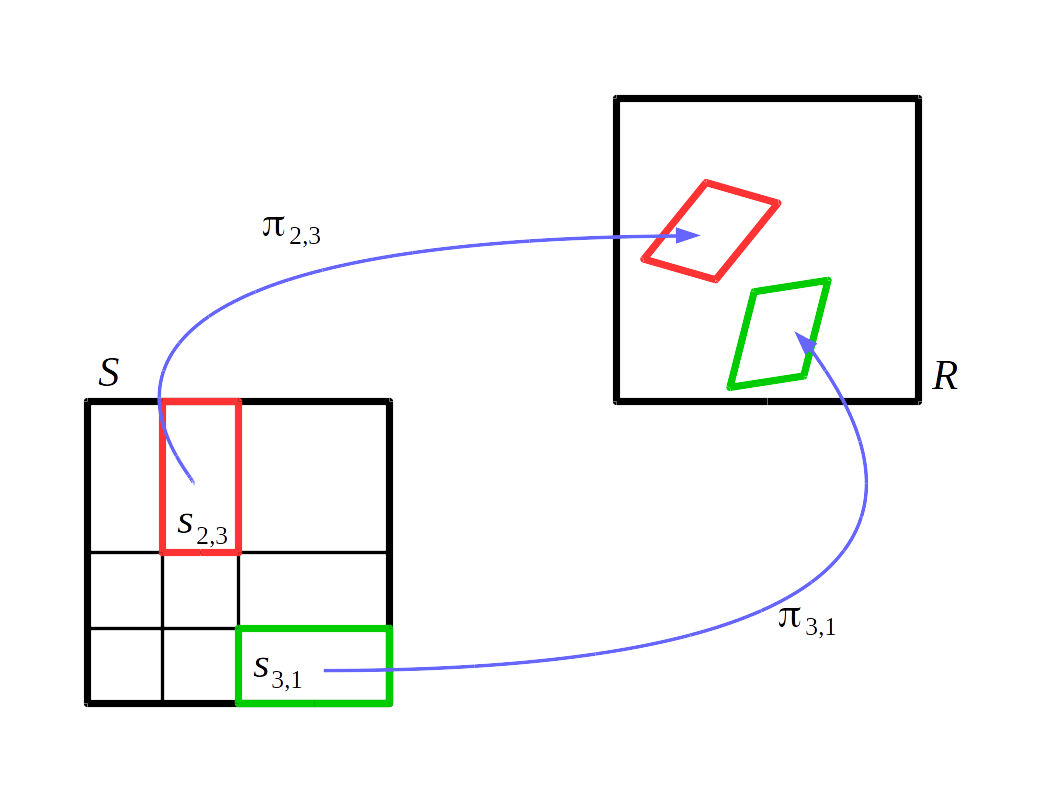
\includegraphics[trim = 0cm 2.2cm 0cm 2cm, clip, scale=0.25]{reachability.png}
  \caption{Mapping of tile $s_{2,3}$ to $R$ via pattern $\pi_{2,3}$,
and mapping of tile $s_{3,1}$ via  $\pi_{3,1}$.}
 \label{fig:reachability}
\end{figure}

%Actually, as mentioned above,
%we will focus on rectangles $S$  which  \emph{contain}  $R$
%(see Section \ref{ss:extension}).


\subsubsection{Parametric extension of tiling}\label{ss:extension}
In the following, we assume that the set $S$ we are looking for
is a \emph{parametric extension} of $R$, denoted by $R+(a,a)$,
which is defined in the following.

Suppose that $R=R_1\times R_2$ is given
as well as a tiling
${\cal R}={\cal R}_1\times {\cal R}_2=\{r_{i_1}\times r_{i_2}\}_{i_1\in I_1, i_2\in I_2}
=\{r_{i_1,i_2}\}_{i_1\in I_1, i_2\in I_2}$.
Then $R_1$ can be seen as a product of~$n_1$ closed intervals
of the form $[\ell,m]$. Consider a nonnegative real parameter~$a$.
Let $(R_1+a)$ denote the corresponding
product of $n_1$ intervals of the form
$[\ell-a,m+a]$.\footnote{Actually, we will consider in the examples
that $(R_1+a)$ is a product of intervals of
the form $[\ell-a,m]$ where the interval is extended only
at its \emph{lower} end, but the method is strictly identical.}
We define $(R_2+a)$ similarly.
Finally, we define $R+(a,a)$ as $(R_1+a)\times (R_2+a)$.

We now consider that $S$ is a (parametric) superset of~$R$
of the form $R+(a,a)$.
We define a tiling ${\cal S}={\cal S}_1\times{\cal S}_2$
of~$S$ of the form $\{s_{i_1}\times s_{i_2}\}_{i_1\in I_1,i_2\in I_2}$,
which is obtained from
%
${\cal R}={\cal R}_1\times{\cal R}_2=
\{r_{i_1}\times r_{i_2}\}_{i_1\in I_1,i_2\in I_2}$ by a simple extension,
as follows:
%
%Let ${\cal S}=\{s_{i_1,i_2}\}_{i_1\in I_1, i_2\in I_2}
%=\{s_{i_1}\times s_{i_2}\}_{i_1\in I_1, i_2\in I_2}$ be the finite rectangular 
%tiling of $S=R+(a,a)$ obtained from the tiling ${\cal R}$ as follows:
A~tile $r_{i_1}$ (resp.~$r_{i_2}$) of ${\cal R}_1$ (resp. ${\cal R}_2$)
in ``contact''
with $\partial R_1$ (resp.~$\partial R_2$)
is extended as a tile~$s_{i_1}$ (resp.~$s_{i_2}$)
in order to be in contact with~$\partial (R_1+a)$
(resp.~$\partial (R_2+a)$); 
a tile 
``interior'' to~$R_1$ (i.e.,~with no contact with~$\partial R_1$)
is kept unchanged, and coincides with~$s_{i_1}$,
and similarly for~$R_2$. 

We denote the resulting tiling ${\cal S}$ by ${\cal R}+(a,a)$.
We~also denote~$s_{i_1}$ (resp.~$s_{i_2}$)
by~$r_{i_1}+a$ (resp.~$r_{i_2}+a$), even if 
$r_{i_1}$ (resp.~$r_{i_2}$) is ``interior'' to~$R_1$
(resp.~$R_2$).
Likewise, we denote~$s_{i,j}$ by~$r_{i,j}+(a,a)$.
%
Note that a tiling of~$R$ of index set $I_1\times I_2$
induces a tiling of $R+(a,a)$ with the same index set
$I_1\times I_2$, hence the same number of tiles as~$R$, for any $a\geq 0$.
This is illustrated in Figure~\ref{fig:tiling2},
where the tiling of~$R$ is represented with black continuous lines,
and the extended tiling of $R+(a,a)$ with red dashed lines.

\begin{figure}[!h]
  \centering
 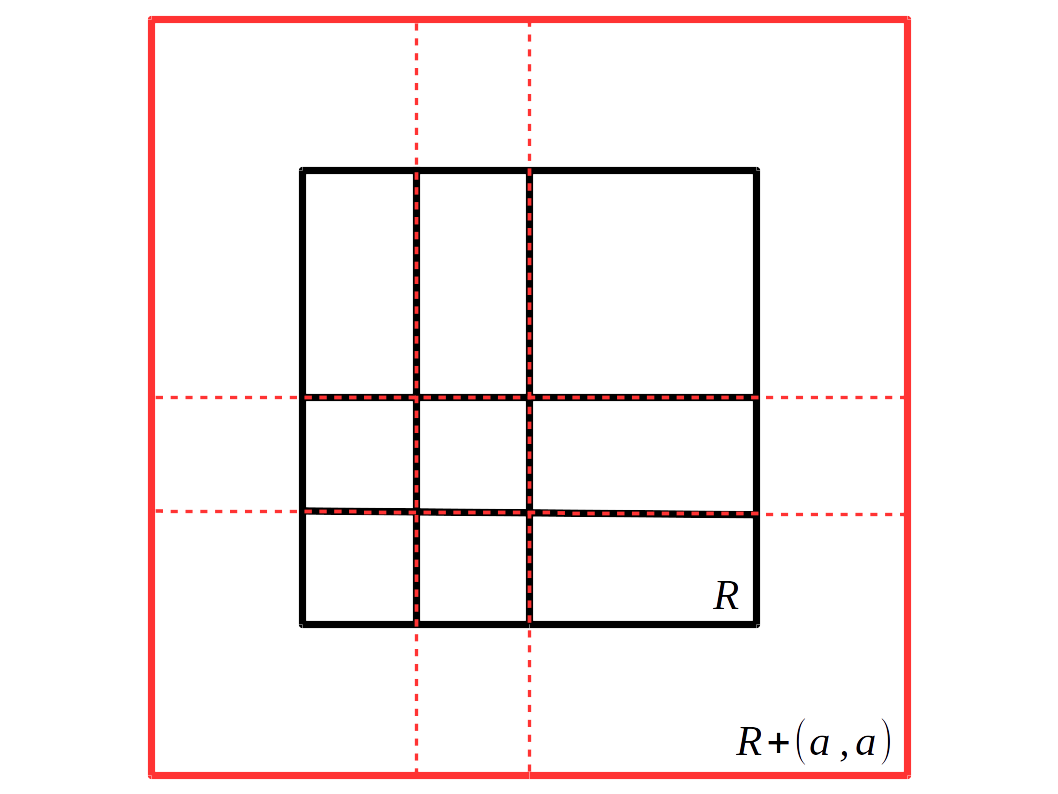
\includegraphics[trim = 0cm 0.3cm 0cm 0.3cm, clip, scale=0.18]{tiling_R.png}
  \caption{Tiling of $R+(a,a)$ induced by tiling ${\cal R}$ of $R$.}
 \label{fig:tiling2}
\end{figure}

\subsubsection{Generate-and-test tilings}\label{ss:gen}
By replacing $S$ with $R+(a,a)$ in the notions defined in
Section~\ref{ss:cent0} %and \ref{ss:dist0},
the problem of macro-step control synthesis can now be reformulated as:
``\emph{find a tiling ${\cal R}$ of~$R$ 
that induces a macro-step 
control of $R+(a,a)$  towards~$R$,  for some $a\geq 0$ (as big as possible)}''.

% besides,
%if we find such ${\cal R}$,
%we want to compute the \emph{maximum} value of $a$
%for which the induced control exists.

This problem can be solved by a simple ``generate-and-test''
procedure: we \emph{generate} a candidate tiling, and then 
\emph{test} if it satisfies the control property (the control test
procedure is explained in Section~\ref{ss:macro_cent}); if the test
fails, we~generate another candidate, and so on iteratively.

In practice, the generation of a candidate~${\cal R}$ is performed
by starting from the trivial tiling (made of one tile equal to~$R$), and
using successive \emph{bisections} of~$R$ until, either the control
test succeeds (``success''), or the depth of bisection of the new
candidate is greater than a given upper bound~$D$ (``failure'').  See
details in~\cite{fribourg2014finite}.%\fbox{+ ref previous papers}

%%%%%  Copie de l'annexe 1

%\fbox{Copie de l'annexe. A reduire un peu...}
\subsubsection{Tiling refinement}\label{ss:refinement}
Let us now explain how we find a tiling ${\cal R}$ of~$R$
such that $\Pi_{i_1,i_2}\neq \emptyset$.
We~focus on the centralized case, but the distributed case is similar.
We~start from the trivial tiling ${\cal R}^0=\{R\}$, which only contains
tile~$R$. If $f(R,\pi)\subseteq R$ for some $\pi\in \Pi^{\leq K}$,
then ${\cal R}^0$ is the desired tiling. Otherwise,
we~refine ${\cal R}^0$ by \emph{bisection}, which gives
a tiling ${\cal R}^1$ of the form $\{r_{(i,1),(j,2)}\}_{1\leq i,j\leq n}$.
If, for all $1\leq i,j\leq n$ there exists some $\pi\in \Pi^{\leq K}$ such that
$f(r_{(i,1),(j,2)},u)\subseteq R$, then ${\cal R}^1$ is the desired tiling.
Otherwise, there exist some ``bad'' tiles of the form $r_{(i,1),(j,2)}$
with $1\leq i,j\leq n$ such that $\forall \pi\in \Pi^{\leq K}\ f(r_{(i,1),(j,2)},\pi)\not\subseteq R$;
we then transform ${\cal R}^1$ into ${\cal R}^2$ by bisecting
all those bad tiles. By iterating this procedure, 
we produce tilings ${\cal R}^1, {\cal R}^2,\cdots, {\cal R}^d$, until
either no bad tiles remain in ${\cal R}^d$ (\emph{success}), 
or the bisection depth~$d$ is greater than
the given upper bound~$D$ (\emph{failure}).
%The treatment of the distributed control is similar.



\subsubsection{Iterated macro-step control synthesis}\label{ss:iteration}
Suppose that we are given an objective rectangle $R=R_1\times R_2$.
If the one-step control synthesis described in
Section~\ref{ss:refinement} succeeds, then there is a nonnegative real
$a^{(1)}=A$ and a tiling~${\cal R}$ of~$R$ that induces a control
steering all the points of $R^{(1)}=R+(a^{(1)},a^{(1)})$ to~$R$ in one
step.  Now the macro-step control synthesis can be reapplied
to~$R^{(1)}$.  If~it succeeds again, then it produces a tiling~${\cal
  R}^{(1)}$ of~$R^{(1)}$ which induces a control that steers
$R^{(2)}=R^{(1)}+(a^{(2)},a^{(2)})$ to~$R^{(1)}$ for some $a^{(2)}\geq
0$.
%in one step.
The iterated application
of macro-step control synthesis outputs a sequence of 
tilings~${\cal R}^{(i)}$,
each of which induces a control that steers 
$R^{(i+1)}=R+(\Sigma_{j=1}^{i+1}a^{(j)},\Sigma_{j=1}^{i+1}a^{(j)})$ 
to~$R^{(i)}$.
%, for some $a^{(j)}\geq 0$ ($1\leq j\leq i+1$).
In~the~end, this~synthesizes a control that steers~$R^{(i+1)}$
to~$R$ in at most $i+1$ macro-steps ($i\geq 0$),
using an increasing sequence of 
nested rectangles around~$R$.
This is illustrated in Figure \ref{fig:iteration}, for $i=1$.


The iteration process halts
at some step, say~$m$, when the last
macro-step control synthesis fails because
the maximum bisection depth~$D$ is reached while ``bad'' tiles still remain
(see~Section~\ref{ss:refinement}). We also stop
the process when the last macro-step control synthesis outputs
a real~$a^{(m)}$ which
is smaller than a given bound: this is because the 
sequence of controllable rectangles around $R$ seems to
approach a limit.


\begin{figure}[t]
  \centering
% 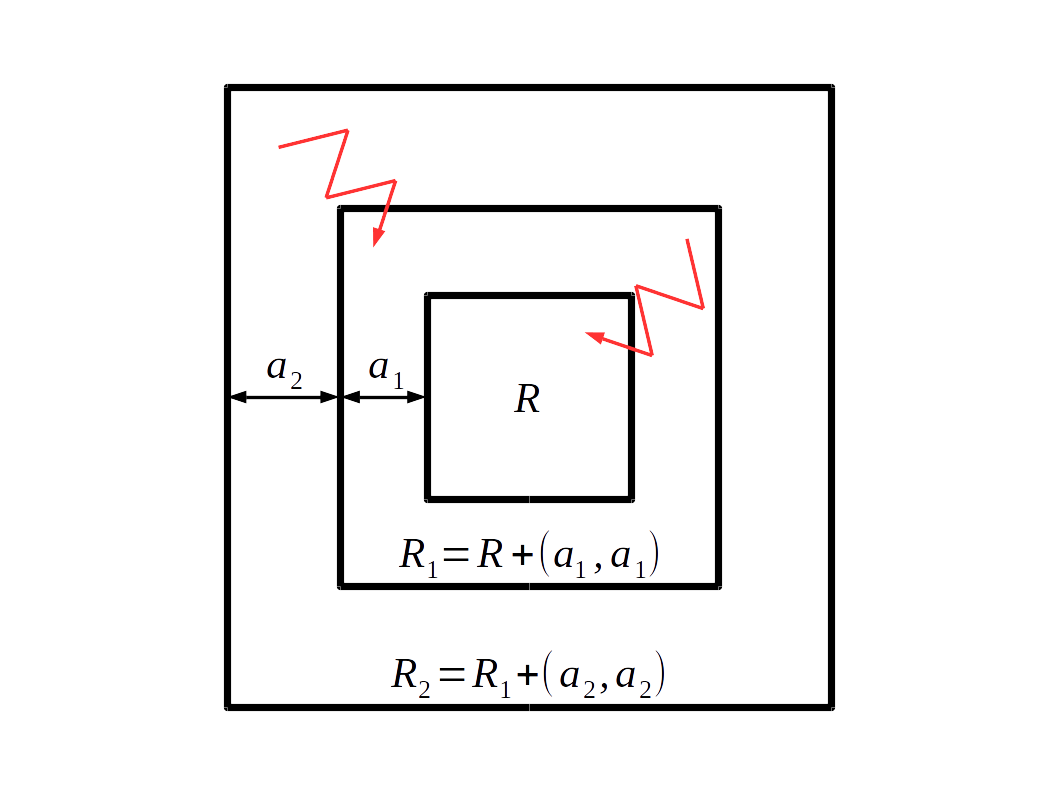
\includegraphics[scale=0.3]{iterated_reachability.png}
 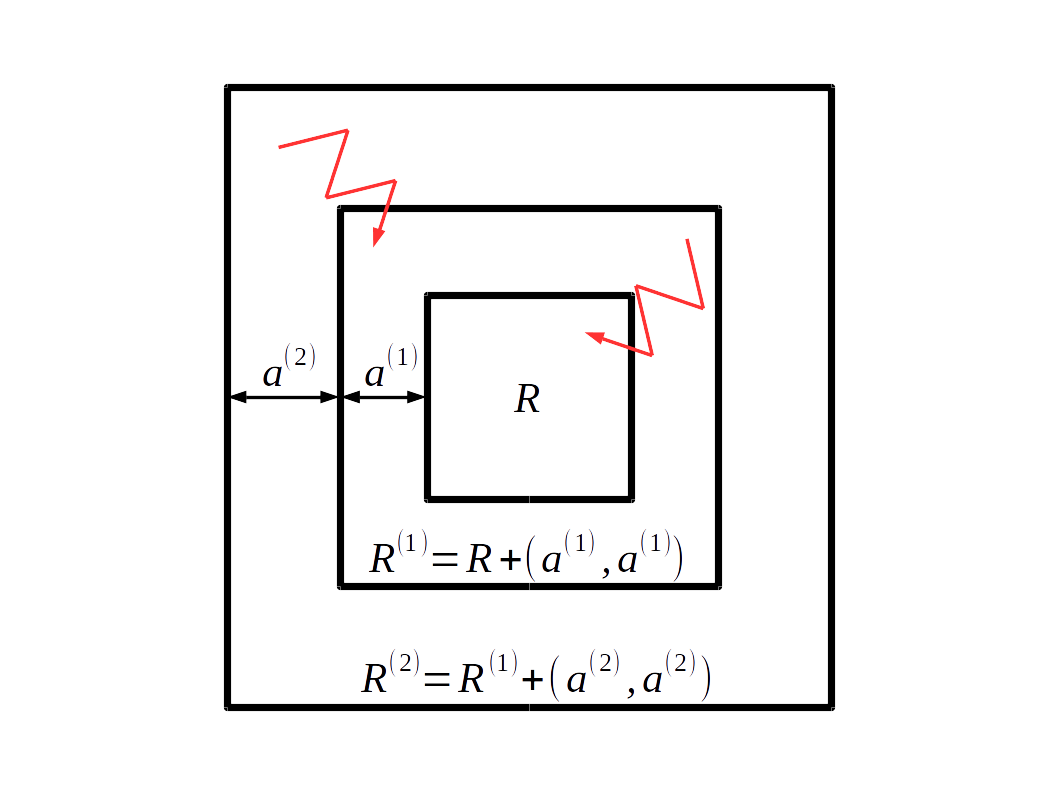
\includegraphics[trim = 0cm 1cm 0cm 1cm, clip, scale=0.25]{tiling_R_iterated.png}
  \caption{Iterated control of $R^{(1)}=R+(a^{(1)},a^{(1)})$ towards $R$,
and $R^{(2)}=R^{(1)}+(a^{(2)},a^{(2)})$ towards $R^{(1)}$.}
 \label{fig:iteration}
\end{figure}


%%%%% fin de l'annexe A1


%\emph{Remark 1.}
\begin{remark}\label{rk1}
Note that, if the generate-and-test process stops with ``success'' for a tiling
${\cal R}$, then the tiling
${\cal R}_{D,uniform}$ also solves the problem,
where ${\cal R}_{D,uniform}$
is the ``finest'' tiling obtained 
by bisecting $D$ times all the $n$ components of $R$.
Since ${\cal R}_{D,uniform}$ has exactly $2^{nD}$ tiles, 
it is in general impractical to perform directly the control test on it.
From a theoretical point of view however, 
it is convenient to suppose that ${\cal R}={\cal R}_{D,uniform}$ 
for reducing the \emph{worst case time complexity }
of the control synthesis procedure to the complexity 
of the control test part only
(see~Section~\ref{ss:macro_cent}).
\end{remark}


\subsection{Centralized control}\label{sec:one-step}
%We consider here 
%that we are given a tiling ${\cal R}$ of $R$
%of the form $\{r_{i_1,i_2}\}_{i_1\in I_1,i_2\in I_2}$.

\subsubsection{Tiling test procedure}\label{ss:macro_cent}

As seen in~Section \ref{ss:extension},
the \emph{(macro-step) 
control synthesis problem with horizon~K} 
consists in finding 
$a\geq 0$ (as big as possible), 
and a tiling ${{\cal R}=\{r_{i_1,i_2}\}_{i_1\in I_1, i_2\in I_2}}$ of~$R$
such that,
%
for each ${(i_1,i_2)\in I_1\times I_2}$,
there exists some~${\pi\in \Pi^{\leq K}}$ 
with
\begin{eqnarray}
f(r_{i_1,i_2}+(a,a),\pi)\subseteq R.
\label{a}
\end{eqnarray}
%
It is easy to see that if~\eqref{a} holds for some $a\geq 0$, then it
also holds for all $a'\leq a$.  In~order to \emph{test} if a tiling
candidate ${\cal R}=\{r_{i_1,i_2}\}_{i_1\in I_1,i_2\in I_2}$ of~$R$
satisfies the desired property, we~define, for each ${(i_1,i_2)\in
I_1\times I_2}$:
\begin{eqnarray}
\Pi_{i_1,i_2}^{\leq K}=\{\pi\in \Pi^{\leq K}\ |\ f(r_{i_1,i_2},\pi)\subseteq R\}.
%\label{a}
\end{eqnarray}
%
%$a_{i_1,i_2}$ by:
Suppose that $\Pi_{i_1,i_2}^{\leq K}\neq\emptyset$. Then we know that
Formula (\ref{a}) is satisfied for $a=0$. In~order to find~$a$ ``as
large as possible'', we~look for the existence of a pattern~$\pi$
such that Formula~\eqref{a} holds also for $a=\frac{|R|}{100}$ and
$a=\frac{|R|}{10}$, where $|R|$ denotes the length of the smallest
side of rectangle~$R$.  Numerous variants of such tests are of course
possible, but such a simple test works well in practice, and we keep
it here for the sake of simplicity.  When $\Pi_{i_1,i_2}^{\leq
  K}\neq\emptyset$, we thus define:
\begin{xalignat*}1
  a_{i_1,i_2} &=
  \max\{a\in\{0,\frac{|R|}{100},\frac{|R|}{10}\}\ |\ \exists \pi\in\Pi^{\leq K}\ 
  f(r_{i_1,i_2}+(a,a),\pi) \subseteq R\}.
 % \\
%  \pi_{i_1,i_2} &=
%%  \mathop{\textrm{argmax}}_{\pi\in\Pi_{i_1,i_2}^{\leq K}}\max\{a\geq 0\mid f(r_{i_1,i_2}+(a,a),\pi)
 %   \subseteq R\}
%    \\
\end{xalignat*}
Suppose that, for all $(i_1,i_2)\in I_1\times I_2$:
$\Pi_{i_1,i_2}^{\leq K}\neq\emptyset$, and
let $A=\min_{(i_1,i_2)\in I_1\times I_2}\{a_{i_1,i_2}\}$.
%
It is easy to see that,
for all $(i_1,i_2)\in I_1\times I_2$, there exists a pattern,
denoted by~$\pi_{i_1,i_2}$, such that:
%
$f(r_{i_1,i_2}+(A,A),\pi_{i_1,i_2}) \subseteq R.$
%




\begin{proposition}
%Let $W=\{W_{i_1}\times W_{i_2}\}_{(i_1,i_2)\in I_1\times I_2}$ be a 
%finite rectangular tiling of R.
%
%Suppose there exists a tiling 
%${\cal R}^0=\{r^0_{i,j}\}_{i\in I_1^0, j\in I_2^0}$
%of $R$ such that:
%$\forall (i,j)\in I_1^0\times I_2^0\ %\exists a\geq 0, 
%\exists \pi\in \Pi^{\leq K}\ 
%f((W_{i_1}+a)\times (W_{i_2}+a),\pi)\subseteq R,$$
%f(r_{i,j},\pi)\subseteq R$.
Suppose that there exists a tiling 
${\cal R}=\{r_{i_1,i_2}\}_{i_1\in I_1, i_2\in I_2}$ of $R$ such that:
%
$$\forall (i_1,i_2)\in I_1\times I_2\ \ \Pi_{i_1,i_2}^{\leq K}\neq \emptyset.$$
%
Then ${\cal R}$ induces
a macro-step control
of horizon $K$ of $R+(A,A)$ towards $R$ with:
%such that, for all $(i_1,i_2)\in I_{1}\times I_2$:
%
$$\forall (i_1,i_2)\in I_1\times I_2:\ 
\ \ f(r_{i_1,i_2}+(A,A),\pi_{i_1,i_2})\subseteq  R$$
%
where $A$ and $\pi_{i_1,i_2}$ are defined as above.
\end{proposition}



For each tile $r_{i_1,i_2}$ of $R$ and each $\pi\in\Pi^{\leq K}$, the
test of inclusion ${f(r_{i_1,i_2},\pi)\subseteq R}$ can be achieved in
time polynomial in~$n$ when $f$ is affine.
%
Hence the test $\Pi_{i_1,i_2}^{\leq K}\neq\emptyset$
can be done in $O(N^K \cdot n^{\alpha})$  
since $\Pi^{\leq K}$ contains $O(N^K)$ elements.
%
%The computation of $\max\{a\geq 0\ | f(r_{i_1,i_2}+(a,a),\pi)\subseteq R\}$
%can be done by \emph{linear programming} in time polynomial in $n$, 
%the dimension of the state space.
%
The computation time of $\{a_{i_1,i_2}\}_{i_1\in I,i_2\in I_2}$, $\pi_{i_1,i_2}$,
and $A$ is thus in $O(N^K \cdot 2^{nD})$, where $D$ is the maximal 
bisection depth.
Hence the complexity of testing
a candidate tiling~${\cal R}$ is in $O(N^K \cdot 2^{nD})$.
By~Remark~\ref{rk1} above, the running time of the 
control synthesis by the generate-and-test procedure is also in 
$O(N^K \cdot 2^{nD})$.
%
%We then have:



Once a candidate tiling ${\cal R}$ satisfying the control test
property is found, the generate-and-test procedure ends with
\emph{success} (see~Section \ref{ss:gen}), and a set
$S=R+(a^{(1)},a^{(1)})$ with $a^{(1)}=A$ has been found.  One can then
\emph{iterate} the ``generate-and-test'' procedure in order to
construct an increasing sequence of nested rectangles of the form
$R+(a^{(1)},a^{(1)})$, $R+(a^{(1)}+a^{(2)},a^{(1)}+a^{(2)})$, $\dots$,
which can all be driven to~$R$. The~process ends at the first step $i\geq 1$ 
for which $a^{(i)}=0$ (no~proper extension of the current
rectangle has been found).
%Appendix~\ref{ss:iteration}.




\begin{example}
\label{ex:ex2}
Consider the specification of a two-room apartment given in Example
\ref{ex:spec}. Set $R=[18.5,22]\times[18.5,22]$.
Let $D=1$ (the depth of bisection is at most 1),
and $K=4$ (the maximum length of patterns is~4).
We look for a centralized controller which will steer
the rectangle $S=[18.5-a,22]\times [18.5-a,22]$
to~$R$ with $a$ as large as possible, and stay in~$R$ indefinitely.
Using our implementation, the computation of the control synthesis
takes 4.14s of CPU time.

The method iterates successfully 15 times the macro-step control synthesis procedure.
We find $S=R+(a,a)$ with $a=53.5$, i.e. $S=[-35,22]\times[-35,22]$.
This means that any element of $S$ can be driven to $R$ within 15 macro-steps
of length (at most) 4, i.e., within $15\times 4=60$
units of time. 
Since each unit of time is of duration
$\tau=5$s, any trajectory starting from $S$ reaches $R$ within $60\times 5=300$s.
Once the trajectory $x(t)$ is in $R$, it returns in $R$
every macro-step of length (at most) 4, i.e., every $4\times 5=20$s.

These results are consistent with the simulation
given in Figure \ref{fig:simu_centralized} for the time evolution
of $(T_1,T_2)$ starting from $(12,12)$.
Simulations of the control, starting from $(T_1,T_2)=(12,12)$,
$(T_1,T_2)=(12,19)$ and $(T_1,T_2)=(22,12)$
are also given in the state space plane
in Figure \ref{fig:simu_centralized}.
\begin{figure}[t]
  \centering
%  \begin{tabular}{cc}
 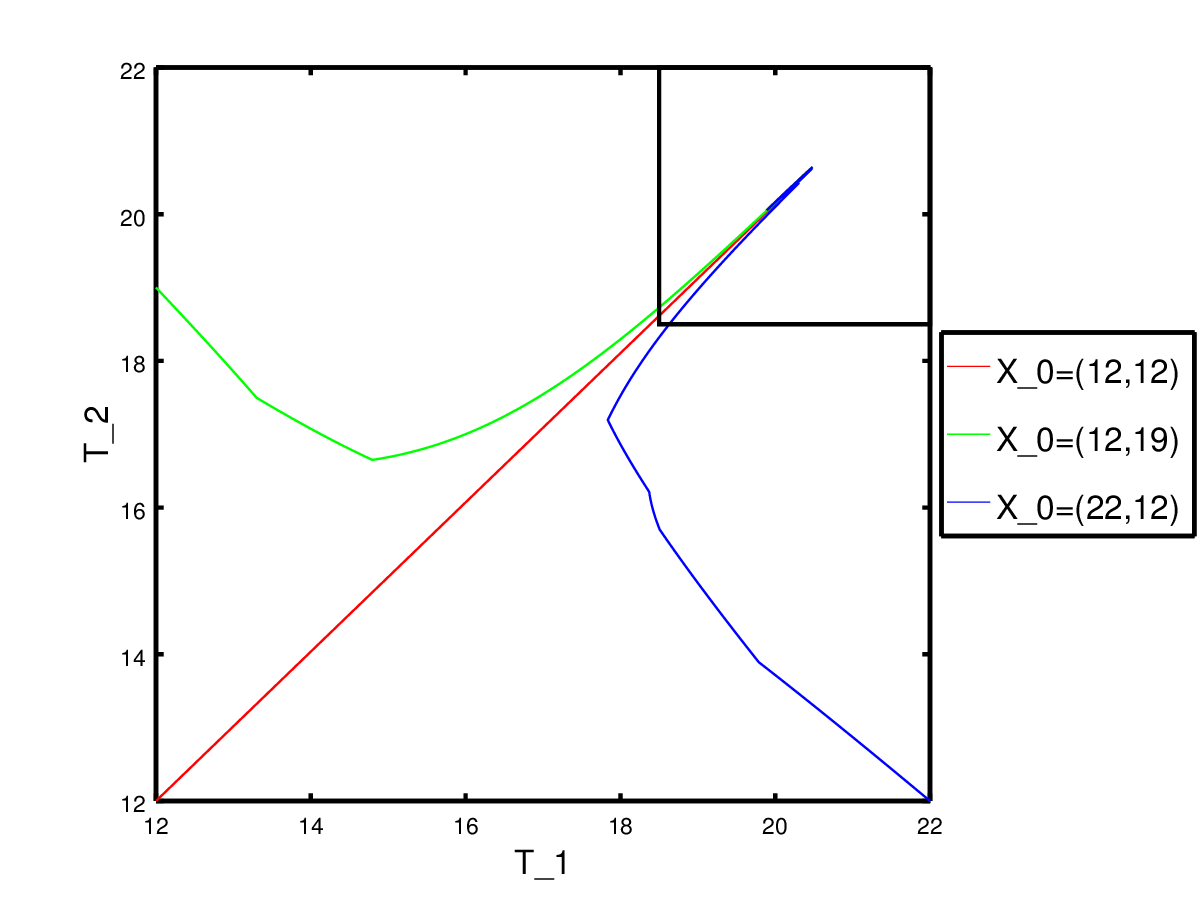
\includegraphics[trim = 0cm 0.3cm 0cm 1cm, clip, width=0.4\textwidth]{simu_2rooms_reach.png} 
% &
\qquad
 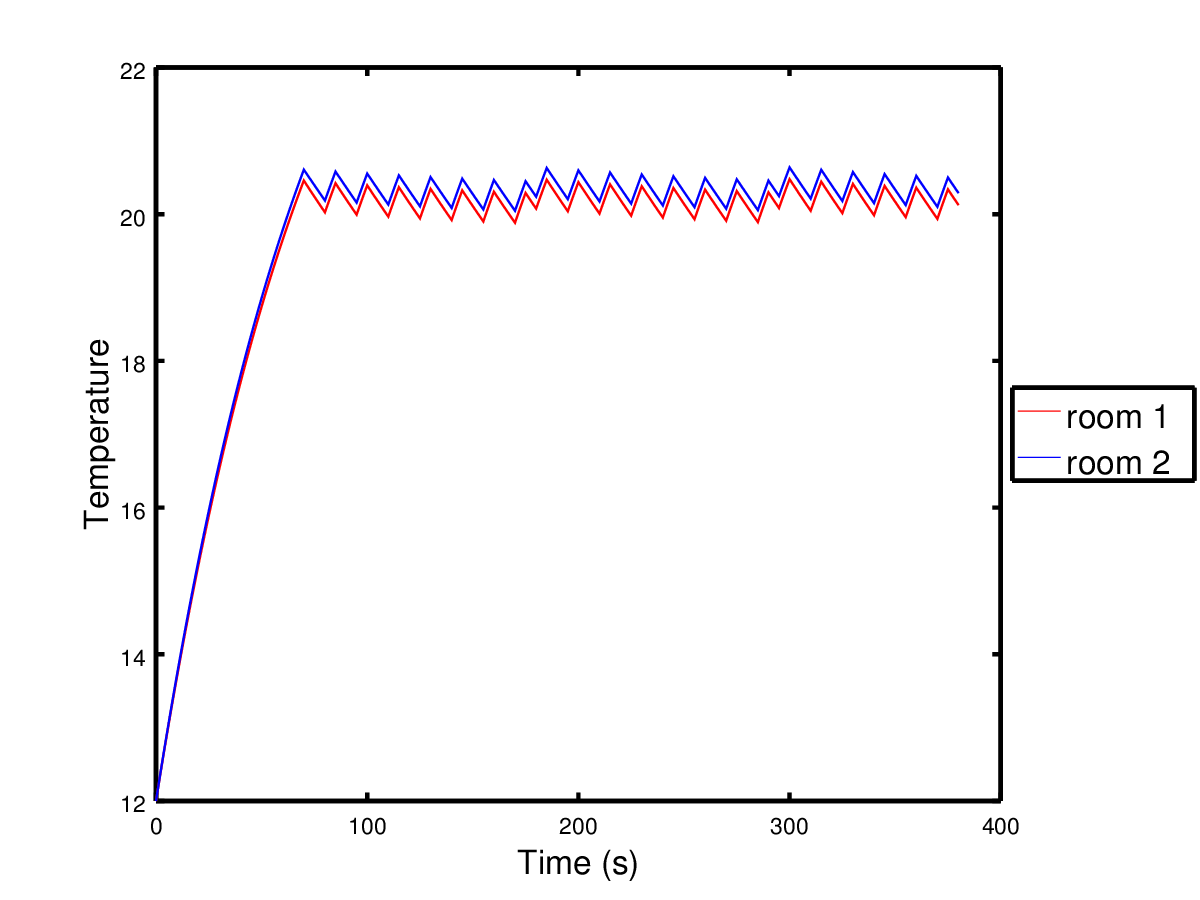
\includegraphics[trim = 0cm 0.3cm 0cm 1cm, clip, width=0.4\textwidth]{simu_centralized_time.png}
%  \end{tabular}

  \caption{Simulations of the centralized reachability controller for
    three different initial conditions plotted in the state space
    plane~(left); simulation of the centralized reachability
    controller for the initial condition $(12,12)$ plotted within
    time~(right).}
  \label{fig:simu_centralized}
\end{figure}
% \begin{figure}[!h]
%   \centering
% 
%   \caption{.}
%  \label{fig:simu_centralized_time}
% \end{figure}
% 
% 
 \end{example}


\subsubsection{Stability as a special case of reachability}\label{ss:special}
Instead of looking for a set of the form $S=R+(a,a)$ from
which $R$ is reachable via a macro-step,
let us consider the particular case where~${S=R}$ (i.e.,~$a=0$).


The problem now consists in constructing a tiling ${\cal
  R}=\{r_{i_1,i_2}\}_{i_1\in I_1, i_2\in I_2}$ of~$R$ such that, for
all $(i_1,i_2)\in I_1\times I_2$, there exists a pattern
$\pi_{i_1,i_2}\in \Pi^{\leq K}$ with ${f(r_{i_1,i_2},
  \pi_{i_1,i_2})\subseteq R}$.  If~such a tiling~${\cal R}$ exists,
then\footnote{If
  $x(t)\in R$, then $x(t)\in r_{i,j}$ for some $(i,j)\in I_1\times
  I_2$, hence $x(t+k)=f(x,\pi_{i,j})\in R$ for some $k\leq K$.}
$x(t)\in R$ implies $x(t+k)\in R$ for some ${k\leq K}$.
Actually, we can slightly modify the procedure in order to
additionally impose that for some $\varepsilon>0$, it~holds $x(t+k')\in
R+(\varepsilon,\varepsilon)$ for any $k'=1,\dots,k-1$
(see~Section~\ref{ss:macro_dist}).  It~follows that $R$ is ``stable''
(with tolerance~$\varepsilon$) under the control induced by~${\cal
  R}$.
%A similar result holds in the distributed context.
%
We can thus treat the stability control of~$R$ 
as a special case  of reachability control.
%with $S=R$ (i.e., $a=0$).





%\section{Macro-steps and Patterns}

\subsection{Distributed control}\label{sec:distr}
\subsubsection{Background}

In the distributed context,
given a set $R=R_1\times R_2$,
the \emph{(macro-step) distributed 
control synthesis problem with horizon~K} 
consists in finding $a\geq 0$, and
a tiling ${\cal R}_1=\{r_{i_1}\}_{i_1\in I_1}$ of $R_1$
which induces a (macro-step) control
on $R_1+a$, a 
tiling ${\cal R}_2=\{r_{i_2}\}_{i_2\in I_2}$
which induces a (macro-step) control on $R_2+a$.

More precisely, we seek tilings ${\cal R}_1$ and ${\cal R}_2$ such that:
%a set $S=S_1\times S_2$ containing $R$ and a tiling
%${\cal  S}_1\times {\cal  S}_2=\{s_{i_1}\}_{i\in I_1}\times\{s_{i_2}\}_{i\in I_2}$ of $S$ such that,
there exists $\ell\in{\mathbb N}$ such
that, for each $i_1\in I_1$ there exists a pattern
$\pi_1$ of $\ell$ modes in $U_1$,
and for each $i_2\in I_2$, 
a pattern $\pi_{2}$ 
of $\ell$ modes in $U_2$ such that:
%
\[
f((r_{i_1}+a)\times (R_2+a),(\pi_1,\pi_2))_{|1}\subseteq R_1 \ \wedge\ 
f((R_1+a)\times (r_{i_2}+a),(\pi_1,\pi_2))_{|2}\subseteq R_2.
\]


In order to synthesize a \emph{distributed} strategy where the control
pattern $\pi_1$ is determined only by $i_1$ (regardless of the value
of $i_2$), and the control pattern $\pi_2$ only by $i_2$ (regardless
of the value of $i_1$), we now define an \emph{over-approximation}
$X_{i_1}(a,\pi_1)$ for
$f((r_{i_1}+a)\times(R_2+a),(\pi_1,\pi_2))_{|1}$, and an
\emph{over-approximation} $X_{i_2}(a,\pi_2)$ for $f((R_1+a)\times
(r_{i_2}+a),(\pi_1,\pi_2))_{|2}$.  The correctness of these
over-approximations relies on the existence of a fixed positive value
for parameter $\varepsilon$.
% parameter 
% $\varepsilon$ of fixed positive real value.
Intuitively, $\varepsilon$ represents the width of
the additional margin (around $R+(a,a)$)
within which all the intermediate states lie when
a macro-step is applied to a point of $R+(a,a)$. 

\subsubsection{Tiling test procedure}\label{ss:macro_dist}

Let $\pi_1^k$ (resp.$\pi_2^k$) denote the prefix of length $k$
of $\pi_1$ (resp.$\pi_2$), and $\pi_1(k)$ (resp. $\pi_2(k)$)
the $k$-th element of pattern $\pi_1$ (resp. $\pi_2$).
\begin{definition}\label{def:1}
Consider an element $r_{i_1}$ (resp. $r_{i_2}$) of a tiling ${\cal
  R}_1$ (resp.~${\cal R}_2$) of~$R_1$ (resp.~$R_2$), and a~pattern
${\pi_1\in\Pi_1^{\leq K}}$ (resp.~${\pi_2\in\Pi_2^{\leq K}}$) of
length~$\ell_1$ (resp.~$\ell_2$).  The \emph{approximate
  first-component (resp. second-component) sequence}
$\{X^k_{i_1}(a,\pi_1)\}_{0\leq k\leq \ell_1}$
(resp. $\{X^k_{i_2}(a,\pi_2)\}_{0\leq k\leq \ell_2}$) is defined as
follows:
\begin{itemize}
\item $X^0_{i_1}(a,\pi_1)=r_{i_1}+a$
  (resp. $X^0_{i_2}(a,\pi_2)=r_{i_2}+a$)
  and 
\item $X^{k}_{i_1}(a,\pi_1)=f_1(X^{k-1}_{i_1}(a,\pi_1),R_2+a+\varepsilon,\pi_1(k))$ for $1\leq k\leq \ell_1$
  (resp. $X^{k}_{i_2}(a,\pi_2)=f_2(R_1+a+\varepsilon,X^{k-1}_{i_2}(a,\pi_2),\pi_2(k))$
for $1\leq k\leq\ell_2$).
%
\end{itemize}
%% (resp. 
%% \begin{itemize}
%% \item $X^0_{i_2}(a,\pi_2)=r_{i_2}+a$ and 
%% \item $X^{k}_{i_2}(a,\pi_2)=f_2(R_1+a+\varepsilon,X^{k-1}_{i_2}(a,\pi_2),\pi_2(k))$
%% for $1\leq k\leq\ell_2$).
%% \end{itemize}
%
\end{definition}
%


We define the property
%
$\Prop_1(a,i_1,\pi_1)$ of $\{X^k_{i_1}(a,\pi_1)\}_{0\leq k\leq \ell_1}$ by:
%$\{X^{k}_1\}_{0\leq k\leq \ell_1}$ such that:
%\begin{itemize}
%\item
\begin{center}
$X^{k}_{i_1}(a,\pi_1)\subseteq R_1+a+\varepsilon$ for $1\leq k\leq \ell_{1}-1$, and
%\item
$X_{i_1}^{\ell_{1}}(a,\pi_1)\subseteq R_1$.
\end{center}
%\end{itemize}
%
Likewise, we define the property
%
$\Prop_2(a,i_2,\pi_2)$ of $\{X^k_{i_2}(a,\pi_2)\}_{0\leq k\leq \ell_2}$ by:
%$\{X^{k}_1\}_{0\leq k\leq \ell_1}$ such that:
%\begin{itemize}
%\item
\begin{center}
$X^{k}_{i_2}(a,\pi_2)\subseteq R_2+a+\varepsilon$ for $1\leq k\leq \ell_{2}-1$, and
  %\item
$X_{i_2}^{\ell_{2}}(a,\pi_2)\subseteq R_2$.
\end{center}
  %\end{itemize}
%
Figure \ref{fig:Q1} illustrates property $\Prop_1(a,i_1,\pi_1)$
for $\pi_1=(u_1\cdot v_1)$,
$\ell_1=2$ and a given tile $r_{i_1}$ with $i_1 \in I_1$:
 $\Prop_1(a,i_1,\pi_1)$ is satisfied because
$X_1^1(a,\pi_1)\subseteq R_1+a+\varepsilon$
and $X_1^2(a,\pi_1)\subseteq R_1$  are true.
% in the lower part, $\Prop_1(a,i_1,\pi_1)$
% is satisfied.



\begin{figure}[t]
  \centering
%  \begin{tabular}{cc}
 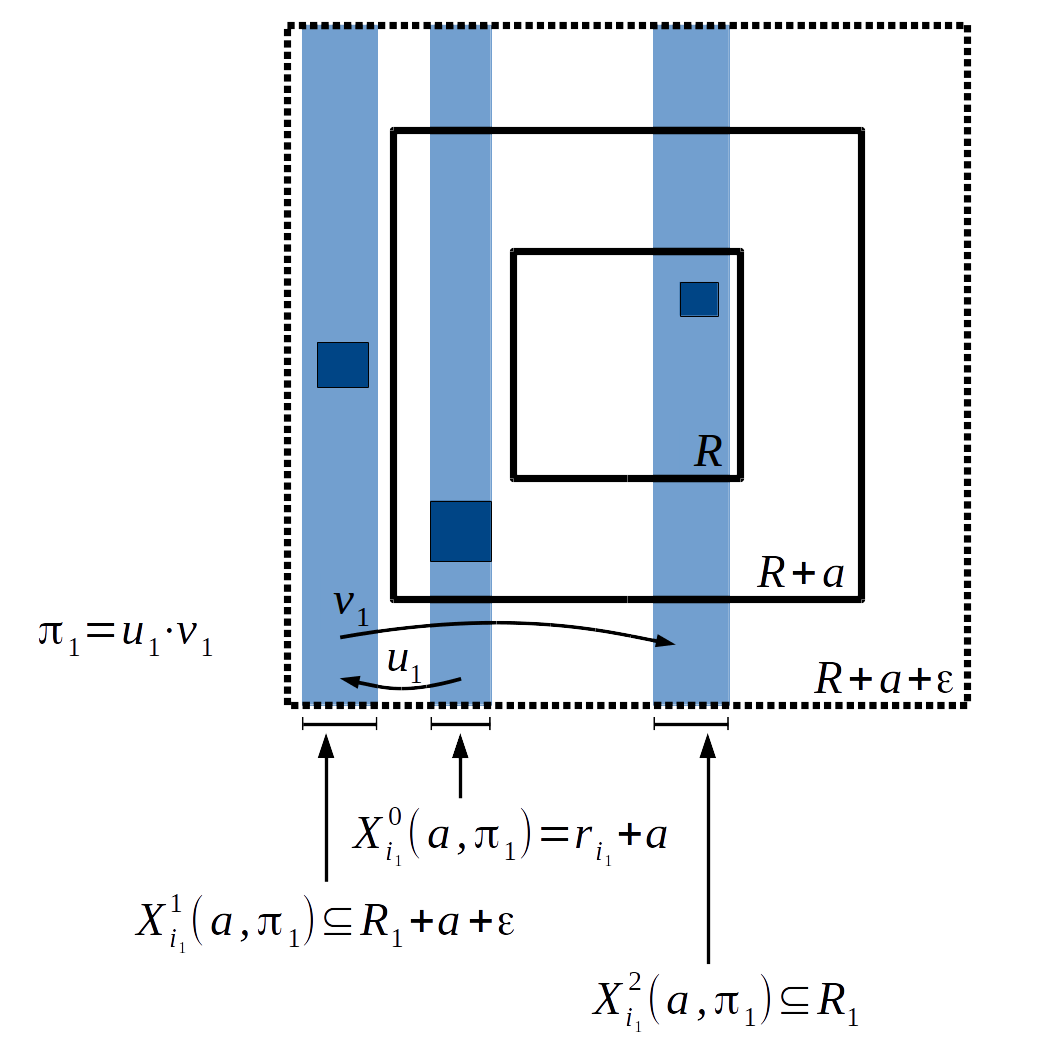
\includegraphics[trim = 0cm 0cm 0cm 0cm, clip, width=0.65\textwidth]{distributed_explanation1.png}
 % &
%  \qquad
%  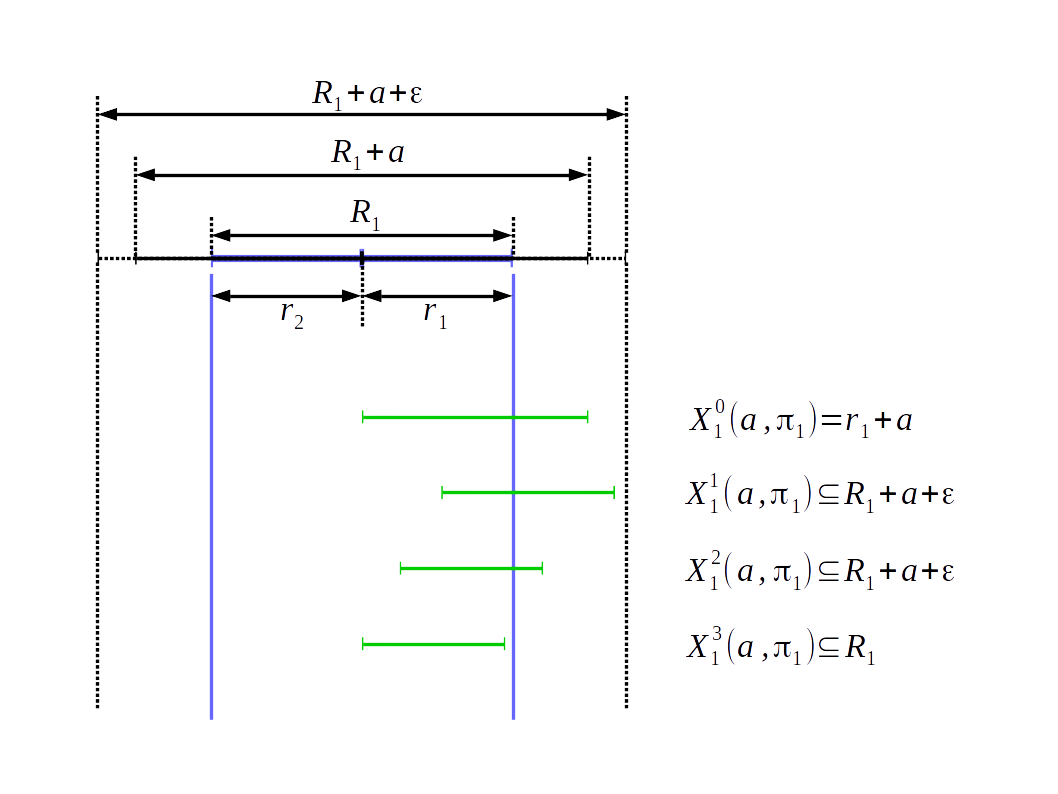
\includegraphics[trim = 2cm 1cm 2cm 2cm, clip, width=0.45\textwidth]{safety_true.png}
%  \end{tabular}

  \caption{Illustration of  $\Prop_1(a,i_1,\pi_1)$  with $i_1 \in I_1$,
$|\pi_1|=\ell_1=2$. The dark blue squares represent the centralized case, where both dimensions
are controlled. The pale blue ribbons represent the distributed case, where we control only
the first dimension, and over-approximate the behavior of the centralized case.}
 \label{fig:Q1}
\end{figure}

\medskip
%Given a tiling ${\cal R}_1=\{r_{i_1}\}_{i_1\in I_1}$  of $R_1$,
%we now define, for each $i_1\in I_1$:
%\[\Pi_{i_1}^{\ell_1}=\{\pi_1\in \Pi_1^{\ell_1}\ |\ 
%\Prop_1(0,i_1,\pi_1)\}.
%\]

Suppose now that there exist $\ell_1$ and $\ell_2$
($1\leq \ell_1,\ell_2\leq K$) such that:
\begin{description}
\item[$H1(\ell_1)$:] 
$\forall i_1\in I_1\  
\exists \pi_1\in \Pi_1^{\ell_1}\  
\Prop_1(0,i_1,\pi_1)$.
%\Pi_{i_1}^{\ell_1}\neq \emptyset$.

\item[$H2(\ell_2)$:] 
$\forall i_2\in I_2\  
\exists \pi_2\in \Pi_2^{\ell_2}\  
\Prop_1(0,i_1,\pi_2)$.
%  $\forall i_2\in I_2\ \Pi_{i_2}^{\ell_2}\neq \emptyset$.
\end{description}
Then we define:
\begin{xalignat*}1
a(\ell_1) & =  \max\{a\in\{0,\frac{|R|}{100},\frac{|R|}{10}\}\mid \forall i_1\in I_1\ \exists \pi_1\in \Pi_1^{\ell_1}\ \Prop_1(a,i_1,\pi_1)\}.
\end{xalignat*}
\begin{xalignat*}1
a(\ell_2) & =  \max\{a\in\{0,\frac{|R|}{100},\frac{|R|}{10}\}\mid \forall i_2\in I_2\ \exists \pi_2\in \Pi_2^{\ell_2}\ \Prop_2(a,i_2,\pi_2)\}.
\end{xalignat*}
Let
$A=\min\{a(\ell_1),a(\ell_2)\}$.
%
From $H1(\ell_1)$-$H2(\ell_2)$, it follows 
that, for all $i_1\in I_1$ there exists
a pattern of~$\Pi_1^{\ell_1}$, denoted by $\pi_{i_1}$, such that
$Prop_1(A,i_1,\pi_{i_1})$, and there exists
a pattern of~$\Pi_2^{\ell_2}$, denoted by $\pi_{i_2}$ such that
$Prop_2(A,i_2,\pi_{i_2})$.

\begin{remark}
  Given a tiling ${\cal R}={\cal R}_1\times{\cal R}_2$, $H1(\ell_1)$ means
  that the points of $R_1+A$ can be (macro-step) controlled to $R_1$
  using patterns which all have the \emph{same length} $\ell_1$; in other
  terms, all the macro-steps controlling $R_1+A$ contain the same
  number $\ell_1$ of elementary steps.  And symmetrically for $H2(\ell_2)$.
\end{remark}
\begin{remark}
  The selection of an appropriate value for~$\varepsilon$ is for the
  moment performed by hand, and is the result of a compromise: if
  $\varepsilon$ is too small, then $f_1(r_{i_1},R_2,\pi_1(1))\subseteq
  R_1+\varepsilon$ for no $\pi_1\in\Pi^{\ell_1}$; if $\varepsilon$ is
  too large, then
  $f_1(X_{i_1}^{\ell_1},R_2+\varepsilon,\pi_1(\ell_1))\subseteq R_1$
  for no $\pi_1\in\Pi^{\ell_1}$.
\end{remark}

%Given a tiling ${\cal R}={\cal R}_1\times{\cal R}_2$ of $R$
%and a real $\varepsilon>0$,
%the problem of existence and computation of
%$k_1$, $k_2$,
%$\{\pi_{i_1}^{k_1}\}_{i_1\in I_1}$,
%$\{\pi_{i_2}^{k_2}\}_{i_2\in I_2}$, and $A$
%can be solved by
%\emph{linear programming} since $f_1$ and $f_2$ are affine.
%
Using the same kinds of calculation as in the centralized case (see
Section~\ref{ss:macro_cent}), one can see that
finding $\ell_1,\ell_2$ such that $\Pi_{i_1}^{\ell_1}\neq \emptyset$
and $\Pi_{i_2}^{\ell_2}\neq \emptyset$,
%checking $H1(\ell_1)$-$H(\ell_2)$,
generating $A$ and $\{\pi_{i_1}\}_{i_1\in I_1}$,
and $\{\pi_{i_2}\}_{i_2\in I_2}$,
can be performed in time $O((\max(N_1,N_2))^K\cdot 2^{\max(n_1,n_2)D})$.
Hence the running time of the control test procedure is also in
$O((\max(N_1,N_2))^K\cdot 2^{\max(n_1,n_2)D})$.

\begin{lemma}\label{prop:lemma}
Consider a tiling ${\cal R}={\cal R}_1\times{\cal R}_2$ of the
form $\{r_{i_1}\times r_{i_2}\}_{(i_1,i_2)\in I_1\times I_2}$.
% Let $i_1\in I_1, i_2\in I_2$ and $a>0$.
%Let $a\geq 0$. 
Suppose that $H1(\ell_1)$ and $H2(\ell_2)$ hold for some
$\ell_1,\ell_2\leq K$.
%, which means that there exists $A\geq 0$ such that for all
%$i_1 \in I_1$, $\Prop_1(A,i_1,\pi_{1})$ holds for some $\pi_{1}\in
%\Pi_1^{\ell_1}$, and for all $i_2 \in I_2$, $\Prop_2(A,i_2,\pi_{2})$
%holds for some $\pi_{2}\in \Pi_2^{\ell_2}$. 
Then we have:

\begin{itemize}
\item in case $\ell_1\leq \ell_2$: for all $1\leq k\leq \ell_1$ and all $i_1\in I_1$,
\begin{xalignat*}1
  f((r_{i_1}+A) \times (R_2+A),(\pi_{i_1}^k,\pi_{i_2}^k))_{|1}
   & \subseteq X_{i_1}^k(A,\pi_{i_1}) \subseteq R_1+A+\varepsilon 
\\
f((R_1+A)\times(r_{i_2}+A),(\pi_{i_1}^k,\pi_{i_2}^k))_{|2}
&\subseteq X_{i_2}^k(A,\pi_{i_2})\subseteq R_2+A+\varepsilon
%\tag{for all $1\leq k\leq \ell_1$}
\\
f((r_{i_1}+A)\times( R_2+A),(\pi_{i_1}^{\ell_1},\pi_{i_2}^{\ell_1}))_{|1}
   &\subseteq X_{i_1}^{\ell_1}(A,\pi_{i_1})\subseteq R_1
\end{xalignat*}

\item in case $\ell_2 \leq \ell_1$: for all $1\leq k\leq \ell_2$ and all $i_2\in I_2$,
  \begin{xalignat*}1
    f((r_{i_1}+A)\times( R_2+A),(\pi_{i_1}^k,\pi_{i_2}^k))_{|1}
      &\subseteq X_{i_1}^k(A,\pi_{i_1})\subseteq R_1+A+\varepsilon
    \\
    f((R_1+A)\times(r_{i_2}+A),(\pi_{i_1}^k,\pi_{i_2}^k)){|_2}
    &\subseteq X_{i_2}^k(A,\pi_{i_2})\subseteq R_2+A+\varepsilon
    \\
%\hspace*{\fill}for all $1\leq k\leq \ell_2$, and
    f((R_1+A)\times(r_{i_2}+A),(\pi_{i_1}^{\ell_2},\pi_{i_2}^{\ell_2}))_{|2}
      &\subseteq X_{i_2}^{\ell_2}(A,\pi_{i_2})\subseteq R_2.
  \end{xalignat*}


\end{itemize}

\end{lemma}
%
%The proof is given in Appendix \ref{sec:proof}.
%\fbox{mettre la preuve ici ?}

\begin{proof}
Suppose $\ell_1 \leq \ell_2$, and
denote by $P_{i_1}^1(k)$ the property
\begin{equation*}
(f((r_{i_1}+A,R_2+A),(\pi_{i_1}^k,\pi_{i_2}^k)))_1 \subseteq X_{i_1}^k
 \label{eq:firstinc}
\end{equation*}
and by $P_{i_1}^2(k)$
\begin{equation*}
X_{i_1}^k \subseteq R_1 + A + \varepsilon
 \label{eq:secondinc}
\end{equation*}
and similarly for $P_{i_2}^1(k)$ and $P_{i_2}^2(k)$.

We show by induction on~$k$ the following property~$P(k)$:
\begin{equation*}
\forall i_1 \in I_1, \ P_{i_1}^1(k) \wedge  P_{i_1}^2(k) \quad \text{and} \quad \forall i_2 \in I_2, \ P_{i_2}^1(k) \wedge  P_{i_2}^2(k). 
\end{equation*}

Let us first consider the case $k = 1$.  Let us prove $\forall i_1 \in
I_1, \ P_{i_1}^1(k) \wedge P_{i_1}^2(k)$ (the~proof is similar for
$\forall i_2 \in I_2, \ P_{i_2}^1(k) \wedge P_{i_2}^2(k)$).  Let us
show that $(f((r_{i_1}+A,R_2+A),(\pi_{i_1}^k,\pi_{i_2}^k)))_1
\subseteq X_{i_1}^k$ and $X_{i_1}^k \subseteq R_1 + A + \varepsilon$.

For $k = 1$,
$\pi_{i_1}^k$ and $\pi_{i_2}^k$ are of the form $u_1$ and $u_2$. We have:
\begin{enumerate}
 \item $(f((r_{i_1}+A,R_2+A),(\pi_{i_1}^k,\pi_{i_2}^k)))_1 = f_1(r_{i_1} + a, R_2 + a, u_1)$
 \item $X_{i_1}^1 = f_1(X_{i_1}^0,R_2 + A + \varepsilon, u_1) = f_1(r_{i_1} + a ,R_2 + A + \varepsilon, u_1) $
\end{enumerate}

Hence $(f((r_{i_1}+A,R_2+A),(\pi_{i_1}^k,\pi_{i_2}^k)))_1 \subseteq X_{i_1}^k$ holds
for $k=1$. And $X_{i_1}^k \subseteq R_1 + A + \varepsilon$ because 
of $\Prop_1(A,i_1,\pi_{i_1})$. 




Let us now suppose that $k>1$ and that $P(k-1)$ holds. We~prove~$P(k)$.
Properties $P_{i_1}^2(k)$ and $P_{i_2}^2(k)$ are true for all $i_1,i_2$ because, 
by~construction, the sequence $X_{i_1}^k$ (resp. $X_{i_2}^k$)
satisfies $\Prop_1(a,i_1,\pi_{i_1})$ (resp. $\Prop_2(a,i_2,\pi_{i_2})$).
Let us prove $P_{i_1}^1(k)$ and $P_{i_2}^1(k)$:

\begin{xalignat*}1
  (f(r_{i_1} +A,R_2+A,(\pi_{i_1}^k,\pi_{i_2}^k)))_1 & = (f(f((r_{i_1}+A,R_2+A),(\pi_{i_1}^{k-1},\pi_{i_2}^{k-1})),\\
  \noalign{\hfill$(\pi_{i_1}{(k)},\pi_{i_2}{(k)})))_1$}
  & =  f_1(\lbrack f((r_{i_1}+A,R_2+A),(\pi_{i_1}^{k-1},\pi_{i_2}^{k-1})) \rbrack, \\
 \noalign{\hfill$\lbrack f((r_{i_1}+A,R_2+A),(\pi_{i_1}^{k-1},\pi_{i_2}^{k-1})) \rbrack
,\pi_{i_1}{(k)})$.} 
\end{xalignat*}
 
 Note that  the first argument of $f_1$ in the last expression satisfies
  $\lbrack f((r_{i_1}+A,R_2+A),(\pi_{i_1}^{k-1},\pi_{i_2}^{k-1}))\rbrack \subseteq X_{i_1}^k $
  by $P_{i_1}^1(k-1)$. Besides, the second argument
  satisfies $\lbrack f((r_{i_1}+A,R_2+A),(\pi_{i_1}^{k-1},\pi_{i_2}^{k-1})) \rbrack
  \subseteq \bigcup_{j_2 \in I_2}X_{j_2}^{k-1} \subseteq R_2 + A + \varepsilon$, because 
  \begin{enumerate}
   \item $r_{i_1} + A \subseteq R_{1}+A$
%    \item $R_2 + a = \bigcup_{j_2 \in I_2} r_{j_2}$
   \item $\bigcup_{j_2 \in I_2} X_{j_2}^{k-1} \subseteq R_2 + A + \varepsilon$ since $X_{j_2}^{k-1} \subseteq R_2 + A + \varepsilon$ \quad (by $P_{j_2}^2(k-1)$ which holds for all $j_2$)
   \item $\lbrack f((R_1 + A , r_{j_2} + A), (\pi_{i_1}^{k-1}, \pi_{i_2}^{k-1})) \rbrack 
  \subseteq X_{j_2}^{k-1}$ \quad (by $P_{j_2}^1(k-1)$).
  \end{enumerate}
  

%   $r_{i_1} + a \subseteq R_{1}+a$ and $R_2 + a = \bigcup_{j_2 \in I2} r_{j_2}$,
%   and $X_{i_2}^{k-1} \subseteq R_2 + A + \varepsilon$ (this is $P_{i_2}^2(k-1)$)
%   and $\lbrack f((R_1 + a , r_{j_2} + a), (\pi_{i_1}(k-1), \pi_{i_2}(k-1))) \rbrack
%   \subseteq X_{j_2}^{k-1}$.
 
 
 Hence 
 \begin{eqnarray*}
  f_1(\lbrack f((r_{i_1}+A,R_2+A),(\pi_{i_1}^{k-1},\pi_{i_2}^{k-1})) \rbrack,\lbrack f((r_{i_1}+A,R_2+A),(\pi_{i_1}^{k-1},\pi_{i_2}^{k-1})) \rbrack,\pi_{i_1}^{(k)} ) \\
  \subseteq f_1(X_{i_1}^{k-1},R_2 + A + \varepsilon,\pi_{i_1}(k)) = X_{i_1}^k
 \end{eqnarray*}

 
 We have thus proved $P_{i_1}^1(k)$:
 \begin{equation*}
 (f(r_{i_1} +A,R_2+A,(\pi_{i_1}^k,\pi_{i_2}^k)))_1 \subseteq X_{i_1}^k
\end{equation*}
This completes the proof of $\forall i_1 \in I_1,\  P_{i_1}^1(k) \wedge P_{i_1}^2(k)$
We prove $P_{i_2}^1(k) \wedge P_{i_2}^2(k)$ for all $i_2 \in I_2$ 
similarly, which concludes the proof of~$P(k)$.
%
The proof of
$(f((r_{i_1}+A,R_2+A),(\pi_{i_1}^{\ell_1},\pi_{i_2}^{\ell_1})))_1
\subseteq X_{i_1}^{\ell_1}(a,\pi_{i_1}) \subseteq R_1$ is similar.
% Note that 
% 
% , and we have
% $X_{i_1}^1 = f_1(X_{i_1}^0,R_2 + A + \varepsilon, u_1) = f_1(r_{i_1} + a ,R_2 + A + \varepsilon, u_1) $
% 
\end{proof}



At $t=0$, consider a point $x(0)=(x_1(0),x_2(0))$ of $R+(A,A)$,
and let us apply concurrently the strategy induced by ${\cal R}_1$
on $x_1$, and ${\cal R}_2$ on $x_2$.
After $\ell_1$ steps, by Lemma \ref{prop:lemma}, we obtain a point 
$x(\ell_1)=(x_1(\ell_1),x_2(\ell_1))\in R_1\times (R_2+A+\varepsilon)$.
Then, after $\ell_1$ steps,
we obtain again a point 
$x(2\ell_1)\in R_1\times (R_2+A+\varepsilon)$,
and so on iteratively.
Likewise, we obtain
points $x(\ell_2), x(2\ell_2),\dots$ which all belong to
$(R_1+A+\varepsilon)\times R_2$.
%
It follows that, after $\ell=lcm(\ell_1,\ell_2)$ steps, we obtain
a point $x(\ell)$ which belongs to $R_1\times R_2=R$.













\begin{theorem}\label{th:1_part3}
%Suppose that there is a tiling ${\cal R}={\cal R}_1\times{\cal R}_2$ 
%of $R$ of the
%form $\{r_{i_1}\times r_{i_2}\}_{(i_1,i_2)\in I_1\times I_2}$.
Suppose that there is a tiling ${\cal R}_1=\{r_{i_1}\}_{i_1\in I_1}$ of $R_1$,
a tiling ${\cal R}_2=\{r_{i_2}\}_{i_2\in I_2}$ of $R_2$,
%Suppose that there is a tiling 
%${\cal R}={\cal R}_1\times{\cal R}_2$ of $R$, 
a positive real $\varepsilon$, and two positive integers $\ell_1,\ell_2\leq K$
such that
$H1(\ell_1)$ and $H2(\ell_2)$ hold.
Let $\ell=lcm(\ell_1,\ell_2)$ with $\ell=\alpha_1 \ell_1=\alpha_2 \ell_2$
for some $\alpha_1,\alpha_2\in \mathbb{N}$.
%Consider the situation described in Proposition \ref{prop:basic}.
%Suppose furthermore that
%$| \pi_{i_1} | = |\pi_{j_1}|=\ell_1$ for all $i_1,j_1\in I_1$, and
%%
%$| \pi_{i_2} | = |\pi_{j_2}|=\ell_2$ for all $i_2,j_2\in I_2$.

Then
%, starting from a point $x=(x_1,x_2)\in (R_1+A)\times (R_2+A)$, 
${\cal R}_1$ induces a 
sequence of $\alpha_1$ macro-steps on $R_1+A$, and ${\cal R}_2$
a sequence of $\alpha_2$ macro-steps on $R_2+A$, such that, 
applied concurrently, we have,
for all $i_1\in I_1$ and $i_2\in I_2$:
%macro-step\footnote{pas exactement ``one'',
%mais $lcm(\ell_1,\ell_2)$ divis\'e par $\ell_1$ and $\ell_2$ respectivement} reachability uniform
%distributed control
%of horizon $K$ 
$$f((r_{i_1}+A)\times (R_2+A),\pi)_{|1}\subseteq R_1 \ \wedge\ 
f((R_1+A)\times (r_{i_2}+A),\pi)_{|2}\subseteq R_2,$$
%$$ f(x,\pi)\in R,$$
%, \mbox{ i.e., } f((x_1,x_2),(\pi_{i_1}^1\cdot \cdots \cdot\pi_{i_1}^{\alpha_1},
%\pi_{i_2}^1\cdot \cdots \cdot\pi_{i_2}^{\alpha_2}))\in R_1\times R_2.$$
for some $\pi=(\pi_1,\pi_2)\in \Pi^{\ell}$ where $\pi_1$ (resp. $\pi_2$)
is of the form $\pi_1^1\cdots \pi_1^{\alpha_1}$
(resp. $\pi_2^1\cdots \pi_2^{\alpha_2}$)
with $\pi_1^i\in \Pi_1^{\ell_1}$  for all $1\leq i\leq \alpha_1$
(resp. $\pi_2^i\in \Pi_2^{\ell_2}$  for all $1\leq i\leq \alpha_2$).
%

Hence:
$$f(r_{i_1,i_2}+(A,A),\pi)\subseteq R.$$
%
Besides, for all prefix $\pi'$ of $\pi$, we have:
$$f((r_{i_1}+A)\times (R_2+A),\pi')_{|1}\subseteq R_1+A+\varepsilon \ \wedge\ 
f((R_1+A)\times (r_{i_2}+A),\pi')_{|2}\subseteq R_2+A+\varepsilon.$$
%
%$$f(x,\pi')\in R+(A+\varepsilon,A+\varepsilon).$$
Hence:
$$f(r_{i_1,i_2}+(A,A),\pi')\subseteq R+(A+\varepsilon,A+\varepsilon).$$
\end{theorem}
%Given the uniform tilings ${\cal R}_{1,D,uniform}$ of $R_1$
%and ${\cal R}_{2,D,uniform}$ of $R_2$,
%on can see along the same lines as in Section \ref{ss:macro_cent},
%that the complexity of 
%checking (H1)-(H2), and computing $A$, $\ell_1$, $\ell_2$, 
%$\{\pi_{i_1}^{\ell_1}\}_{i_1\in I_1}$ and $\{\pi_{i_2}^{\ell_2}\}_{i_2\in I_2}$
%is in $O(\max(N_1,N_2)^K \cdot 2^{\max(n_1,n_2) D})$.\\
%(see Appendix \ref{sec:affine}???).\\

If $H1(\ell_1)$-$H2(\ell_2)$ hold, there exists a control that
steers $R+(A,A)$ to $R$ in $\ell$ steps.
Letting $R^{(1)}=R+(A,A)$, it is then possible to iterate the process
on $R^{(1)}$ and, in case of success, 
to generate a rectangle $R^{(2)}=R^{(1)}+(A^{(1)},A^{(1)})$ 
from which $R^{(1)}$ would be
reachable in $\ell'$ steps, for some $A^{(1)}\geq 0$ and $\ell'\in\mathbb{N}$.
And so on, iteratively, one generates
an increasing  sequence of nested control rectangles,
as in Section~\ref{ss:macro_cent}, until a step $i$ for which 
$A^{(i)}=0$.
%as explained in Section \ref{ss:iteration}.

Theorem \ref{th:1_part3} allows us to implement the method as far as we are able to compute the results of applying mappings $f_1$ and $f_2$ to symbolic states represented by rectangles. 
When $f_1$ and $f_2$ are affine, the results
can be easily computed using the data structure of
``zonotopes'' \cite{Girard05}. The method has been implemented in the case of affine
mappings, using the system MINIMATOR~\cite{minimator,fribourg2014finite}.


\begin{example}
Consider again the specification of a two-room apartment given in
Example \ref{ex:spec}.  We consider the distributed control synthesis
problem where the first (resp.~second) state component corresponds to
the temperature of thefirst (resp.~second) room~$T_1$ (resp.~$T_2$),
and the first (resp.~second) control mode component corresponds to the
heater~$u_1$ (resp.~$u_2$) of the the first (resp.~second) room.

Set $R=R_1\times R_2=[18.5,22]\times[18.5,22]$.
Let $D=3$ (the depth of bisection is at most 3),
and $K=10$ (the maximum length of patterns is 10).
The parameter $\varepsilon$ is set to value $1.5^\circ C$.
We look for a distributed controller 
which steers any temperature state
in $S=S_1\times S_2=[18.5-a,22]\times [18.5-a,22]$
to~$R$ with $a$ as large as possible, 
then maintain it in~$R$ indefinitely.

Using our implementation, the computation of the control synthesis
takes 220s of CPU time.
%
The method iterates 8 times the macro-step control synthesis
procedure.  We find $S=[18.5-a,22]\times [18.5-a,22]$ with $a=6.5$,
i.e.  $S=[12,22]\times[12,22]$.  This means that any element of $S$
can be driven to $R$ within 8 macro-steps of length (at~most) 10,
i.e., within $8\times 10=80$ units of time.  Since each unit of time
is of duration $\tau=5$s, any trajectory starting from~$S$ reaches~$R$
within $80\times 5=400$s.  The trajectory is then guaranteed to always
stay (at~each discrete time~$t$) in
$R+(\varepsilon,\varepsilon)=[17,23.5]\times[17,23.5]$.

These results are consistent with the simulation given in
Figure~\ref{fig:simu_distri} showing the time evolution of $(T_1,T_2)$
starting from $(12,12)$.  Simulations of the control are also given in
the state space plane, in Figure~\ref{fig:simu_distri}, for initial
states $(T_1,T_2)=(12,12)$, $(T_1,T_2)=(12,19)$ and
$(T_1,T_2)=(22,12)$.

Not surprisingly, the performance guaranteed by the distributed
approach ($a = 6.5$, reachability of $R$ in $400$s) are worse than
those guaranteed by the centralized approach of Example \ref{ex:ex2}
($a=53.5$, reachability of $R$ in~$300$s).  However, unexpectedly, the
CPU computation time in the distributed approach ($220$s) is here
worse than the CPU time of the centralized approach ($4.14$s). This
relative inefficiency is due to the small size of the example.

\begin{figure}[t]
  \centering
%  \begin{tabular}{cc}
   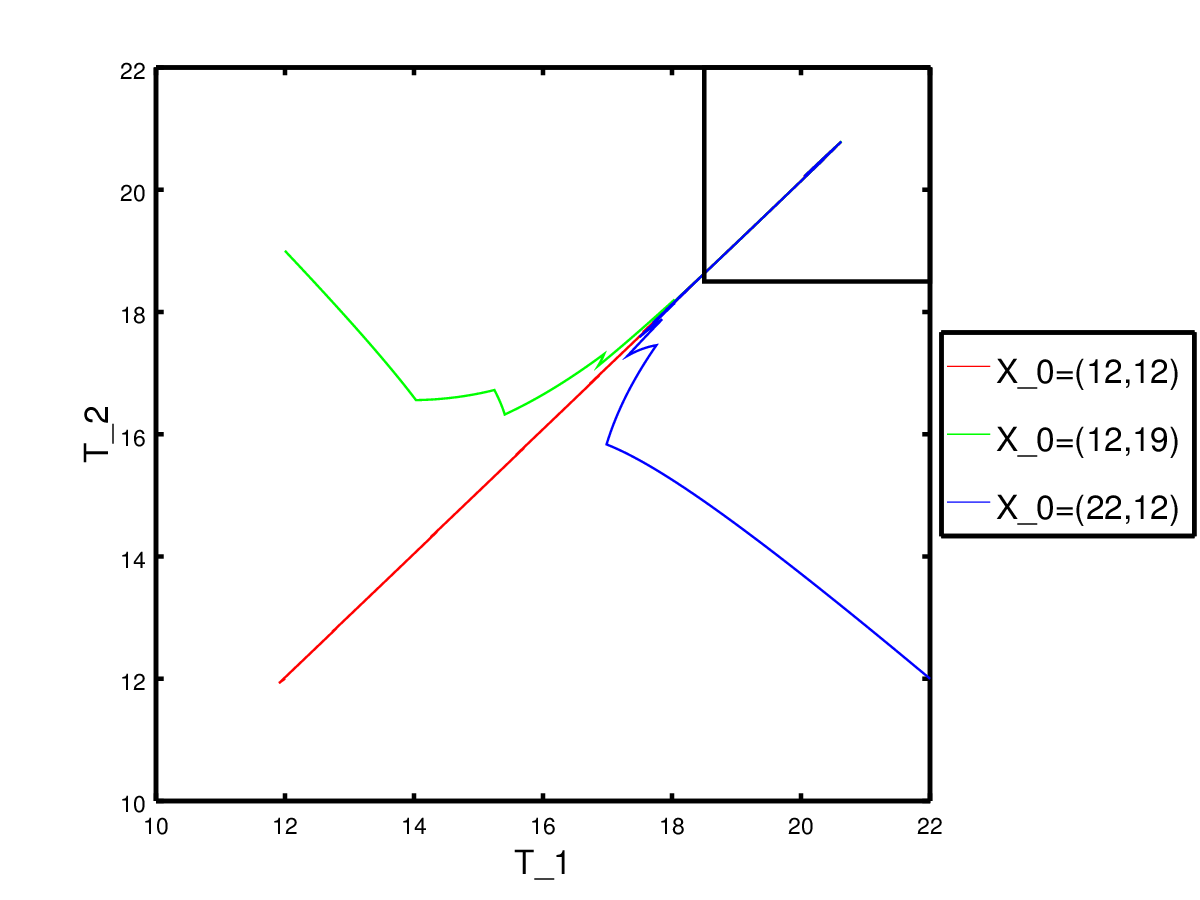
\includegraphics[trim = 0cm 0.3cm 0cm 1cm, clip, width=0.4\textwidth]{simu_distributed_2rooms_state.png}
%   &
\qquad
   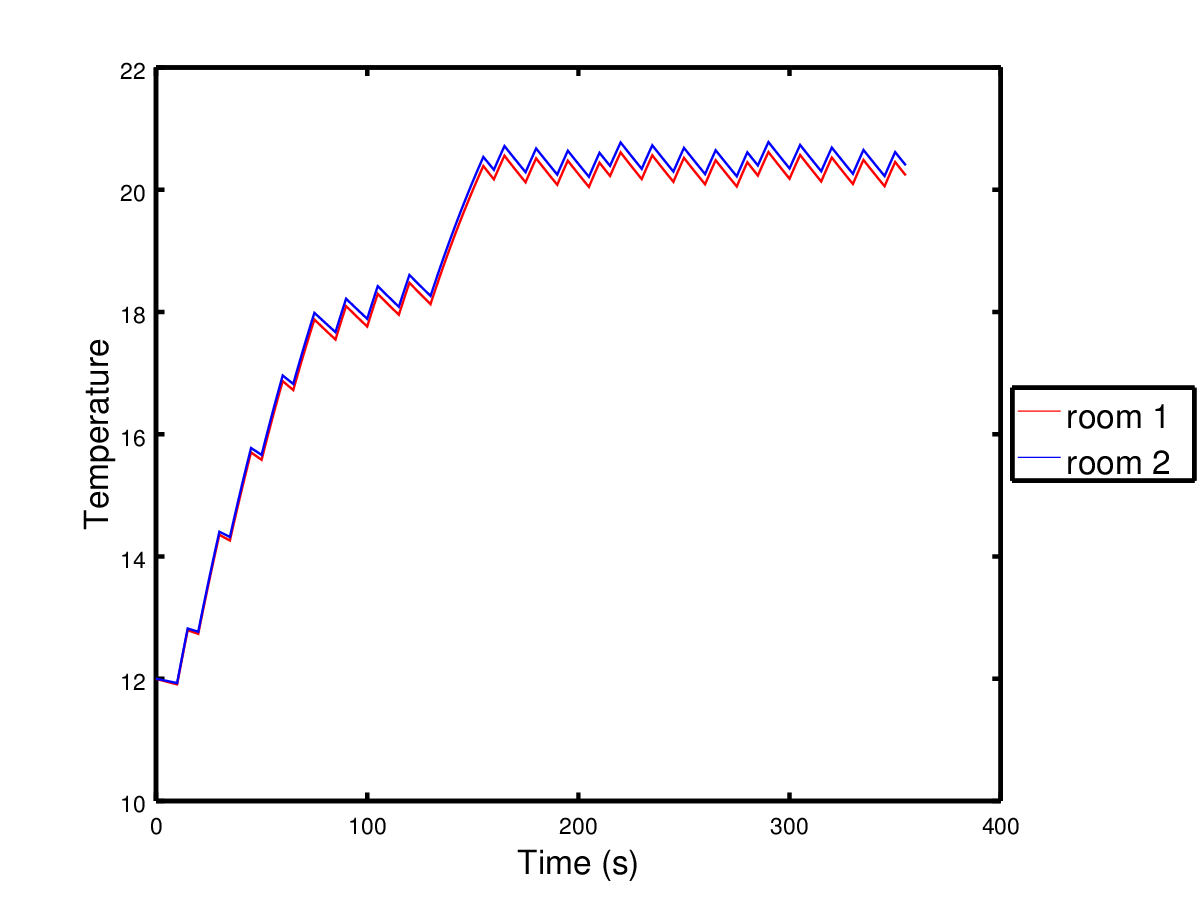
\includegraphics[trim = 0cm 0.3cm 0cm 1cm, clip, width=0.4\textwidth]{simu_distributed_2rooms_time.png}
%  \end{tabular}

  \caption{Simulations of the distributed reachability controller for three different initial conditions plotted
  in the state space plane (left); simulation of the distributed reachability controller for the initial condition $(12,12)$ plotted 
  within time (right).}
 \label{fig:simu_distri}
\end{figure}

% \begin{figure}[!h]
%   \centering
% 
%   \caption{.}
%  \label{fig:simu_distri_time}
% \end{figure}
% 
 \end{example}

%\section{Case where $f_1$ and $f_2$ are affine}

\subsection{Case Study}
\label{sec:case_study0}

This case study, proposed by the Danish company Seluxit, aims at controlling 
the temperature of an eleven rooms house, heated by geothermal energy.
%We manage to synthesize a correct-by-construction control for this 
%example.
The~\emph{continuous} dynamics of the system is the following:
\begin{equation}
 \frac{d}{dt} T_i(t) = \sum_{j=1}^n A_{i,j}^d (T_j(t) - T_i(t)) + B_i(T_{env} (t) - T_i(t)) + H_{i,j}^v.v_j 
\end{equation}



The temperatures of the rooms are the $T_i$.  The matrix $A^d$
contains the heat transfer coefficients between the rooms, matrix $B$
contains the heat transfer coefficients betweens the rooms and the
external temperature, set to ${T_{env} = 10^\circ C}$ for the
computations. The~control matrix~$H^v$ contains the effects of the
control on the room temperatures, and the control variable is here
denoted by~$v_j$. We~have $v_j = 1$ (resp.~$v_j = 0$) if the heater in
room~$j$ is turned on (resp.~turned~off). We~thus have $n=11$ and
$N=2^{11} = 2048$ switching modes.


Note that the matrix $A^d$ is parametrized by the open of closed state
of the doors in the house. In our case, the average between closed and
open matrices was taken for the computations. The exact values of the
coefficients are given in~\cite{larsen2015online}.  The controller has
to select which heater to turn on in the eleven rooms. Due to a
limitation of the capacity supplied by the geothermal device, the~$11$
heaters cannot be turned on at the same time.  In~our case, we~limit
to~$4$ the number of heaters that can be on at the same time.


%--------
We consider the distributed control synthesis problem where
the first (resp. second) state component corresponds to 
the temperatures of rooms~1 to~5 (resp.~6 to~11),
and the first (resp. second) control mode component corresponds to the heaters 
of rooms~1 to~5 (resp.~6 to~11).
Hence $n_1=5, n_2=6, N_1=2^5, N_2=2^6$. We~impose
that at most two heaters are switched on at the same time in the
first sub-system, and at most two in the second sub-system.

Let $D=1$ (the bisection depth is at most~1),
and $K=4$ (the maximum length of patterns is~4).
The parameter $\varepsilon$ is set to value $0.5^\circ C$.
The sampling time is $\tau=15$ minutes.


We look for a distributed controller 
which steers any temperature state in
the rectangle $S=[18-a,22]^{11}$
to $R=[18,22]^{11}$ with $a$ as large as possible, 
then maintain the temperatures in~$R$ indefinitely.
%
Using our implementation, the computation of the control synthesis
takes around 20 hours of CPU time.
%
The method iterates the macro-step control synthesis procedure 15
times.  We~find $S=[18-a,22]^{11}$ with $a=4.2$, i.e.
$S=[13.8,22]^{11}$.  This means that any element of~$S$ can be driven
into~$R$ within 15 macro-steps of length (at~most)~4, i.e., within
$15\times 4=60$ units of time.  Since each time unit is of duration
$\tau=15$ min, any trajectory starting from~$S$ reaches~$R$ within
$60\times 15=900$ min.  The~trajectory is then guaranteed to stay in
$R+(\varepsilon,\varepsilon)=[17.5,22.5]^{11}$.
%
These results are consistent with the simulation given in
Figure~\ref{fig:reach_11rooms_10} showing the time evolution of the
temperature of the rooms, starting from~$14^{11}$.

%Robustness simulations for our controller
%are given in Appendix \ref{sec:robustness}.



\begin{figure}[t]
  \centering
 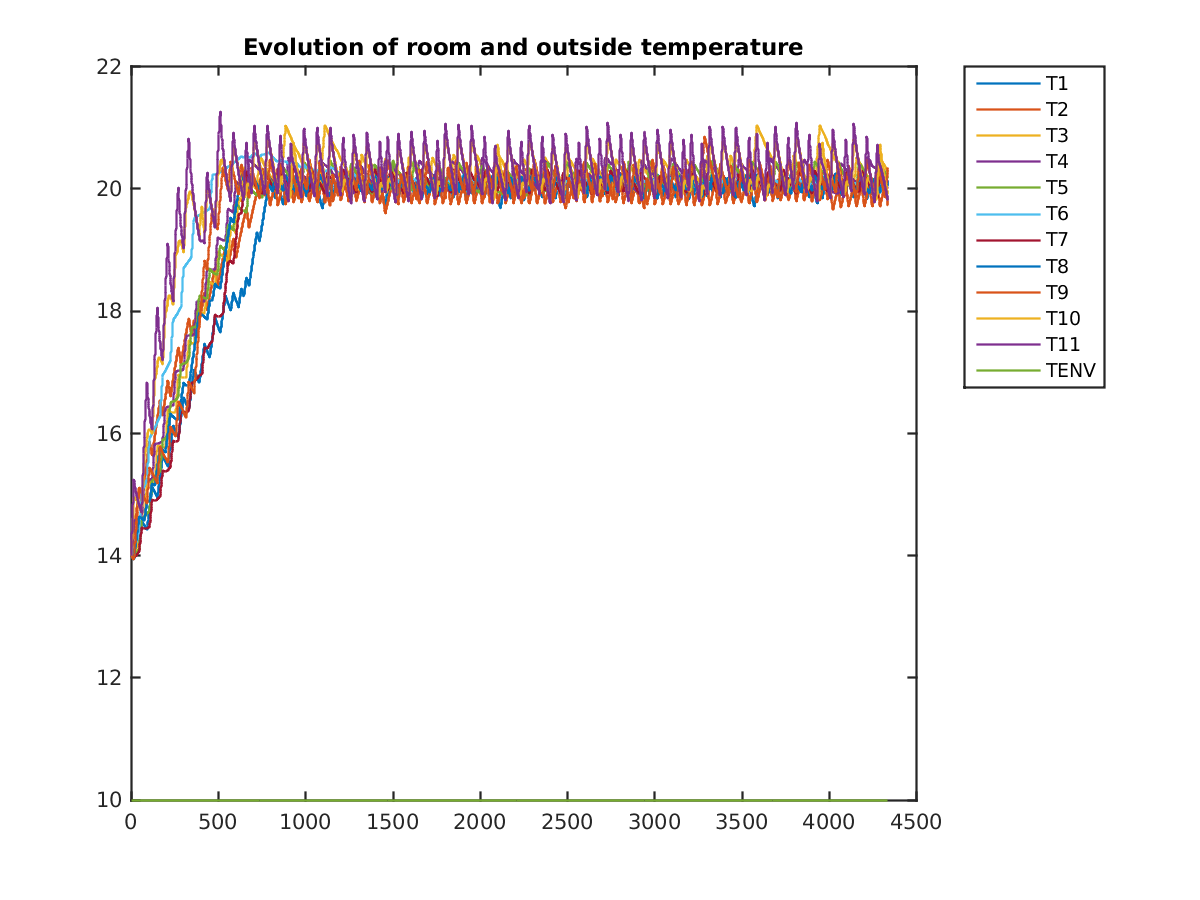
\includegraphics[trim = 0cm 1cm 0cm 0cm, clip, scale = 0.4]{reachability_11rooms_synchronized_10_degrees.png}
 \caption{Simulation of the Seluxit case study 
plotted with time (in min) for $T_{env}=10^{\circ} C$.}
 \label{fig:reach_11rooms_10}
\end{figure}



\subsubsection{Robustness Experiments}\label{sec:robustness}


We now perform the same simulations as in Figure \ref{fig:reach_11rooms_10}, except 
that the environment temperature is not fixed at $10^\circ$C but follows
scenarios of soft winter (Figure~\ref{fig:reach_11rooms}) and spring 
(Figure \ref{fig:reach_11rooms_stab}). The environment temperature is plotted
in green in the figures. The spring scenario is taken from \cite{larsen2015online},
and the soft winter scenario is the winter scenario 
of \cite{larsen2015online} with $5$ additional degrees.
We see that our controller, which is designed for $T_{env} = 10^\circ$C still
satisfies the properties of reachability and stability. These simulations 
are very close those obtained in~\cite{larsen2015online}.

\begin{figure}[ht]
  \centering
 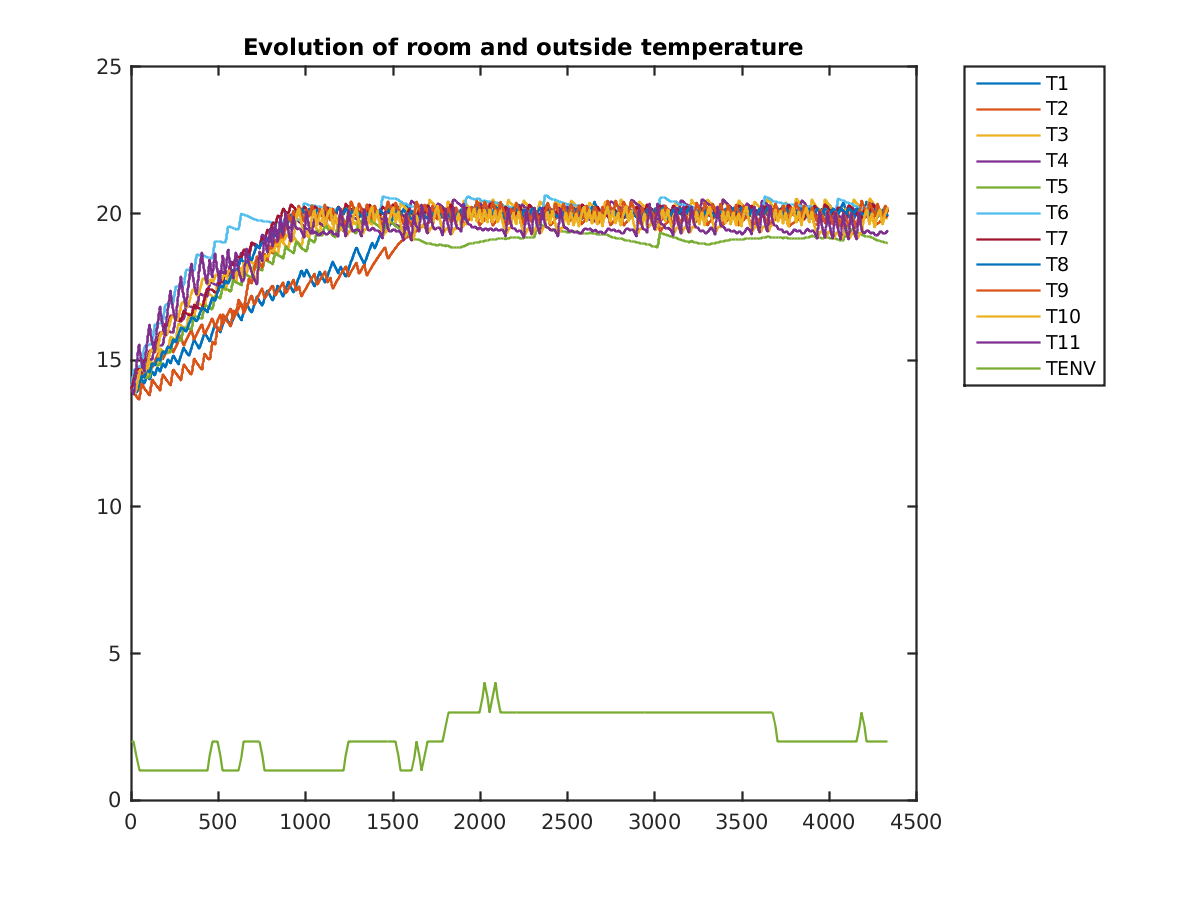
\includegraphics[trim = 0cm 1cm 0cm 0cm, clip, scale = 0.4]{reachability_11rooms.png}
 \caption{Simulation of the Seluxit case study in the soft winter scenario.}
 \label{fig:reach_11rooms}
\end{figure}


\begin{figure}[ht]
  \centering
 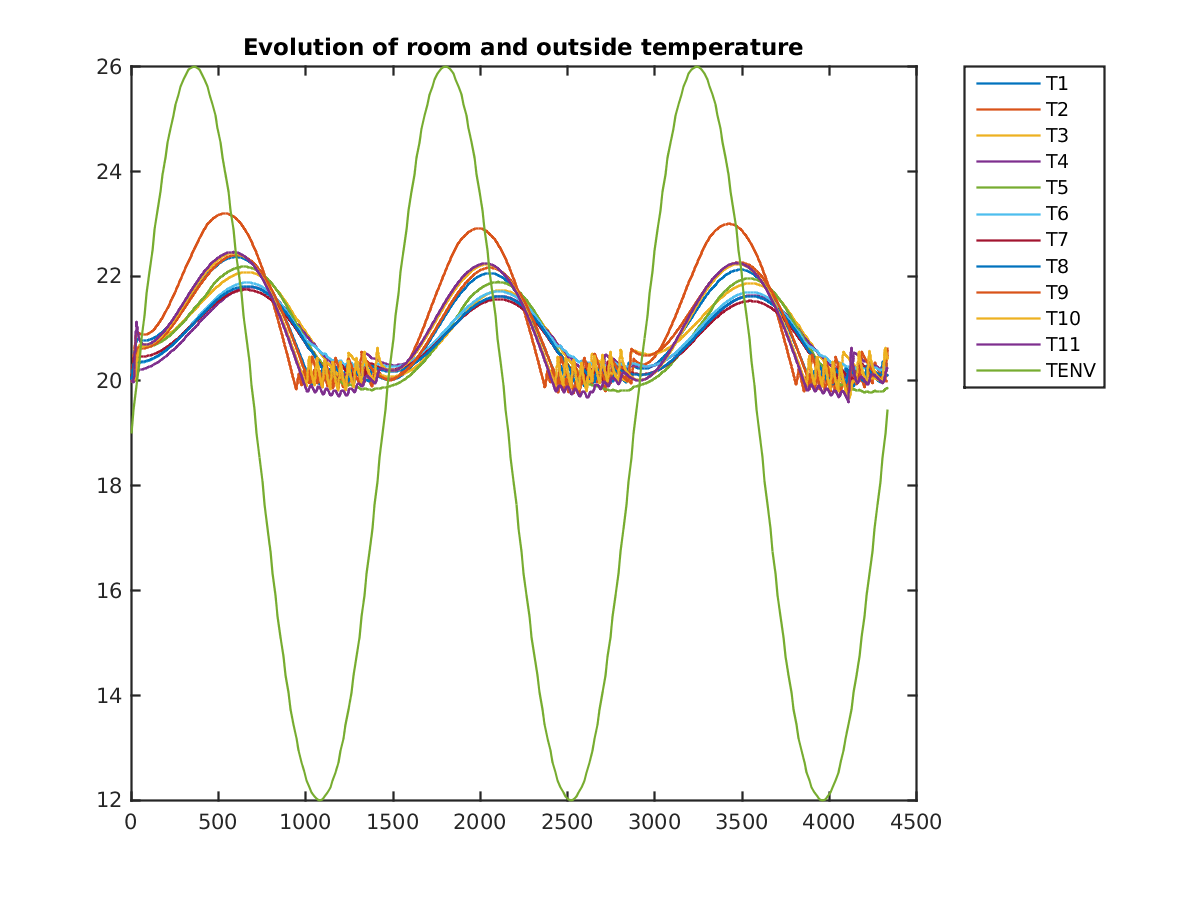
\includegraphics[trim = 0cm 1cm 0cm 0cm, clip, scale = 0.4]{stability_11rooms.png}
 \caption{Simulation of the Seluxit case study in the spring scenario.}
 \label{fig:reach_11rooms_stab}
\end{figure}

%%%%% fin copie de l'annexe









\subsection{Continuous-time case}
%\label{sec-nonilnear}
\label{sec-continuous}
In this section, we consider the case of continuous-time differential equations.
The~time~$t$ now takes its value in~$\mathbb{R}_{\geq 0}$.
\subsection{Reachability in continuous time}
Consider the continuous-time system with \emph{finite control}:
\begin{xalignat}1
 \dot{x}_1(t) &= f_1(x_1(t),x_2(t),u_1) \label{eq:nl_sys1} \\
 \dot{x}_2(t) &= f_2(x_1(t),x_2(t),u_2) 
 \label{eq:nl_sys2}
\end{xalignat}
where $x_1$ (resp.~$x_2$) is the first (resp. second)  component
of the state vector variable, taking its values
in $\mathbb{R}^{n_1}$ (resp.~$\mathbb{R}^{n_2}$), 
and where $u_1$ (resp.~$u_2$) is
the first (resp.~second) component of the control \emph{mode},
taking its values in the \emph{finite} set~$U_1$ (resp.~$U_2$).
We will often write~$x$ for $(x_1,x_2)$, $u$~for~$(u_1,u_2)$,
and $n$ for~$n_1+n_2$.
We will also abbreviate the set $U_1\times U_2$ as~$U$.
%
%Let $N$ be the cardinal of $U$, and $N_1$ (resp. $N_2$) the cardinal
%of $U_1$ (resp. $U_2$). We have $N=N_1 \cdot N_2$.
%
We~abbreviate the continuous-time system under
the form:
%
\begin{equation}
\dot{x}(t)=f(x(t),u)
\label{eq:nl_sys_central}
\end{equation}
%
where $x$ is a vector state variable taking its values in
$\mathbb{R}^n=\mathbb{R}^{n_1}\times \mathbb{R}^{n_2}$, and where
$u$~is of the form $(u_1,u_2)$, with $u_1$ taking its values in $U_1$
and $u_2$ in~$U_2$.  We~assume that, given an initial value~$x_0$,
Equation~\eqref{eq:nl_sys_central} has a solution
%
(e.g., assuming that the vector field~$f$ (resp.~$f_1$,~$f_2$) is
Lipschtiz).


We define the reachable set of~\eqref{eq:nl_sys_central} from a set of
initial states $X_0$, at time $t$ $(0\leq t\leq \tau)$ under control
mode~$u$:
%
\[
\Reach_f(t,X_0,u)=\{\Phi(t,x_0,u) \ |\ x_0\in X_0\}.
\]
%
where $\Phi(t, x,u)$ denotes the state $x(t)$ reached at time $t$
$(0\leq t\leq \tau)$ starting from the initial state~$x$, under
control mode $u\in U$.


%\fbox{factoriser les deux paragraphes suivants}
We define the reachable set of \eqref{eq:nl_sys1} from a set of initial states
$X_1\subset \mathbb{R}^{n_1}$, at time $t$ $(0\leq t\leq \tau)$ under control mode $u_1\in U_1$ and perturbation $X_2\subset \mathbb{R}^{n_2}$:
%
\[
\Reach_{f_1}(t,X_1,X_2,u_1)=\{\Phi_1(t,x_1,X_2,u_1) \ |\ x_1\in X_1\}.
\]
%
where
$\Phi_1(t, x_1,X_2,u_1)$ is the set of states $x_1(t)$ reached at time 
$t$ $(t\geq 0)$ from the initial 
state $x_1$, under control mode $u_1$ and perturbation $X_2$.

Symmetrically, we
define the reachable set of \eqref{eq:nl_sys2} from a set of initial states
$X_2\subset \mathbb{R}^{n_2}$, at time $t$ $(0\leq t\leq \tau)$ under control mode $u_2\in U_2$ and perturbation $X_1\subset \mathbb{R}^{n_1}$:
%
\[
\Reach_{f_2}(t,X_1,X_2,u_2)=\{\Phi_2(t,X_1,x_2,u_2) \ |\ x_2\in X_2\}.
\]
%
where
$\Phi_2(t, X_1,x_2,u_2)$ is the set of states $x_2(t)$ reached at time 
$t\geq 0$ from the initial 
state $x_2$, under control mode $u_2$ and perturbation $X_1$.

All the notions of reachable sets for modes are extended in the
natural manner to the notions of reachable sets for \emph{patterns}. 
For example, for the pattern $\pi=u\cdot v$ of
length~$2$, and for $0\leq t\leq \tau$, we~define:
\begin{xalignat*}1
  \Reach_f(t,X_0,\pi) & = \Reach_f(t,X_0,u)
  %\text{ for $0\leq t\leq \tau$
  \\
  \Reach_f(\tau+t,X_0,\pi) & = \Reach_f(t,X_1,v)
  %for $0\leq t\leq \tau$,
 \qquad\text{with $X_1=\Reach_f(\tau,X_0,u)$.}
\end{xalignat*}



%We suppose that we are able to compute an overapproximation
%of the reachable set denoted $\overline{\Reach}$. 




\subsubsection{Distributed control}
Recall that $\pi_1^k$ (resp. $\pi_2^k$) denotes the prefix of length $k$
of $\pi_1$ (resp.$\pi_2$), and $\pi_1(k)$ (resp. $\pi_2(k)$)
the $k$-th element of sequence $\pi_1$ (resp. $\pi_2$).
We now give the counterpart of Definition \ref{def:1}.
\begin{definition}
Consider an element $r_{i_1}$ (resp. $r_{i_2}$) of a tiling ${\cal R}_1$
(resp. ${\cal R}_2$) of $R_1$
(resp. $R_2$), and a sequence $\pi_1\in\Pi_1^{\leq K}$ (resp. $\pi_2\in\Pi_2^{\leq K}$)
of length $\ell_1$ (resp. $\ell_2$).
The \emph{approximate first-component sequence}
$\{Y^k_{i_1}(a,\pi_1)\}_{0\leq k\leq \ell_1}$ 
is defined as follows:
\begin{itemize}
\item $Y^0_{i_1}(a,\pi_1)=r_{i_1}+a$ and 
\item $Y^{k}_{i_1}(a,\pi_1)=\bigcup_{0\leq t\leq \tau}\Reach_{f_1}(t,Y^{k-1}_{i_1}(a,\pi_1),R_2+a+\varepsilon,\pi_1(k))$ for ${1\leq k\leq \ell_1}$.
%
\end{itemize}
Similarly, the \emph{approximate second-component sequence} $\{Y^k_{i_2}(a,\pi_2)\}_{0\leq k\leq \ell_2}$ is defined by
\begin{itemize}
\item $Y^0_{i_2}(a,\pi_2)=r_{i_2}+a$ and 
\item $Y^{k}_{i_2}(a,\pi_2)=\bigcup_{0\leq t\leq \tau}\Reach_{f_2}(t,R_1+a+\varepsilon,Y^{k-1}_{i_2}(a,\pi_2),\pi_2(k))$
for ${1\leq k\leq\ell_2}$.
\end{itemize}
%
\end{definition}
%

We define the property
%
$\Prop_1(a,i_1,\pi_{1})$ by:
%$\{Y^{k}_1\}_{0\leq k\leq \ell_1}$ such that:
%\begin{itemize}
%\item
\begin{center}
  $Y^{k}_{i_1}(a,\pi_{1})\subseteq R_1+a+\varepsilon$ for $1\leq k\leq \ell_{1}$\par
  and
  %\item
  $\Reach_{f_1}(\ell_1\tau,r_{i_1}+a,R_2+a+\varepsilon,\pi_{1})\subseteq R_1$.
\end{center}
%\end{itemize}
%
Likewise, we define the property
%
$\Prop_2(a,i_2,\pi_{2})$ by:
%$\{Y^{k}_1\}_{0\leq k\leq \ell_1}$ such that:
%\begin{itemize}
%\item
\begin{center}
  $Y^{k}_{i_2}(a,\pi_{2})\subseteq R_2+a+\varepsilon$ for $1\leq k\leq \ell_{2}$\par
  and
  %\item
  $\Reach_{f_2}(\ell_2\tau,R_1+a+\varepsilon,r_{i_2}+a,\pi_{2})\subseteq R_2$.
\end{center}
%\end{itemize}

Assumptions $H1(\ell_1)$, $H_2(\ell_2)$ and expressions 
$A$, 
$\pi_{i_1}$, $\pi_{i_2}$
are defined exactly
as in Section~\ref{ss:macro_dist}.
%
We now give the counterpart of Lemma \ref{prop:lemma} 
(the proof is similar).

\begin{lemma}\label{prop:lemma2}
Consider a tiling ${\cal R}={\cal R}_1\times{\cal R}_2$ of the
form $\{r_{i_1}\times r_{i_2}\}_{(i_1,i_2)\in I_1\times I_2}$.
% Let $i_1\in I_1, i_2\in I_2$ and $a>0$.
Suppose that $H1(\ell_1)$ and
$H2(\ell_2)$ hold, for some positive real $\varepsilon$, 
and some positive integers $\ell_1, \ell_2$.
%(i.e: for all $i_1 \in I_1$, $\Prop(a,i_1,\pi_{1})$
%holds for some $\pi_{1}\in \Pi_1^{\ell_1}$, and for all $i_2 \in
%I_2$, $\Prop(a,i_2,\pi_{2})$ holds for some
%$\pi_{2}\in \Pi_2^{\ell_2}$).
Then we have

\begin{itemize}
\item in case $\ell_1\leq \ell_2$, for all $t\in [(k-1)\tau, k\tau]$
($1\leq k\leq \ell_1$):
%\fbox{for all $k\leq \ell_1$ and $t$ such that ... ???}
  \begin{xalignat*}1
  \Reach_f(t,(r_{i_1}+A) \times (R_2+A),(\pi_{i_1}^k,\pi_{i_2}^k))_{|1}\subseteq Y_{i_1}^k(a,\pi_{i_1})
& \subseteq R_1+A+\varepsilon
\\
\Reach_f(t,(R_1+A)\times(r_{i_2}+A),(\pi_{i_1}^k,\pi_{i_2}^k))_{|2}\subseteq Y_{i_2}^k(a,\pi_{i_2})
&\subseteq R_2+A+\varepsilon 
\\
%\hspace*{\fill}for all $1\leq k\leq \ell_1$, and
%
\Reach_f(\ell_1\tau,(r_{i_1}+A)\times( R_2+A),(\pi_{i_1}^{\ell_1},\pi_{i_2}^{\ell_1}))_{|1}%\subseteq Y_{i_1}^{\ell_1}(a,\pi_{i_1})
& \subseteq R_1.
\end{xalignat*}

\item in case $\ell_2 \leq \ell_1$, for all $t \in [(k-1)\tau, k\tau]$
$(1\leq k\leq \ell_2)$:
%\fbox{for all $k\leq \ell_1$ and $t$ such that ... ???}
\begin{xalignat*}1
\Reach_f(t,(r_{i_1}+A)\times( R_2+A),(\pi_{i_1}^k,\pi_{i_2}^k))_{|1}\subseteq Y_{i_1}^{k}(a,\pi_{i_1})
&\subseteq R_1+A+\varepsilon
\\
\Reach_f(t,(R_1+A)\times(r_{i_2}+A),(\pi_{i_1}^k,\pi_{i_2}^k)){|_2}\subseteq Y_{i_2}^k(a,\pi_{i_2})
&\subseteq R_2+A+\varepsilon
\\
%\hspace*{\fill}for all $1\leq k\leq \ell_2$, and
\Reach_f(\ell_2\tau,(R_1+A)\times(r_{i_2}+A),(\pi_{i_1}^{\ell_2},\pi_{i_2}^{\ell_2}))_{|2}%\subseteq Y_{i_2}^{\ell_2}(a,\pi_2)
& \subseteq R_2.
\end{xalignat*}





\end{itemize}

\end{lemma}

We now give the counterpart of Theorem \ref{th:1_part3} (the proof is similar).

\begin{theorem}\label{th:2}
%Suppose that there is a tiling ${\cal R}={\cal R}_1\times{\cal R}_2$ 
%of $R$ of the
%form $\{r_{i_1}\times r_{i_2}\}_{(i_1,i_2)\in I_1\times I_2}$.
Suppose that there is a tiling ${\cal R}_1=\{r_{i_1}\}_{i_1\in I_1}$ of $R_1$
and a tiling ${\cal R}_2=\{r_{i_2}\}_{i_2\in I_2}$ of $R_2$,
%Suppose that there is a tiling 
%${\cal R}={\cal R}_1\times{\cal R}_2$ of $R$, 
%and a positive real $\varepsilon$
such that
$H1(\ell_1)$ and $H2(\ell_2)$ hold
for some $\ell_1,\ell_2 \leq K$.
Let $\ell=lcm(\ell_1,\ell_2)$ with $\ell=\alpha_1 \ell_1=\alpha_2 \ell_2$
for some $\alpha_1,\alpha_2\in \mathbb{N}$.
%Consider the situation described in Proposition \ref{prop:basic}.
%Suppose furthermore that
%$| \pi_{1} | = |\pi_{j_1}|=\ell_1$ for all $i_1,j_1\in I_1$, and
%%
%$| \pi_{2} | = |\pi_{j_2}|=\ell_2$ for all $i_2,j_2\in I_2$.

Then
%, starting from a point $x=(x_1,x_2)\in (R_1+a)\times (R_2+a)$, 
${\cal R}_1$ induces a 
sequence of $\alpha_1$ macro-steps on $R_1+A$, and ${\cal R}_2$
a sequence of $\alpha_2$ macro-steps on $R_2+A$, such that, 
when applied concurrently, we have
for all $i_1\in I_1$ and $i_2\in I_2$:
%macro-step\footnote{pas exactement ``one'',
%mais $lcm(\ell_1,\ell_2)$ divis\'e par $\ell_1$ and $\ell_2$ respectivement} reachability uniform
%distributed control
%of horizon $K$ 
\begin{multline*}
\Reach_f(\ell \tau,(r_{i_1}+A)\times (R_2+A),\pi)_{|1}\subseteq R_1 \ \wedge\\ 
\Reach_f(\ell \tau,(R_1+A)\times (r_{i_2}+A),\pi)_{|2}\subseteq R_2,
\end{multline*}
%$$ f(x,\pi)\in R,$$
%, \mbox{ i.e., } f((x_1,x_2),(\pi_1^1\cdot \cdots \cdot\pi_1^{\alpha_1},
%\pi_2^1\cdot \cdots \cdot\pi_2^{\alpha_2}))\in R_1\times R_2.$$
for some $\pi=(\pi_1,\pi_2)\in \Pi^{\ell}$ where $\pi_1$ (resp. $\pi_2$)
is of the form $\pi_1^1\cdots \pi_1^{\alpha_1}$
(resp. $\pi_2^1\cdots \pi_2^{\alpha_2}$)
with $\pi_1^i\in \Pi_1^{\ell_1}$  for all $1\leq i\leq \alpha_1$
(resp. $\pi_2^i\in \Pi_2^{\ell_2}$  for all $1\leq i\leq \alpha_2$).
%
Hence:
$$\Reach_f(\ell\tau,r_{i_1,i_2}+(A,A),\pi)\subseteq R.$$
Besides, for all $0\leq t \leq \ell\tau$,
we have:
\begin{multline*}
  \Reach_f(t,(r_{i_1}+A)\times (R_2+A),\pi)_{|1}\subseteq R_1+A+\varepsilon\\ 
  \wedge\ \Reach_f(t,(R_1+A)\times (r_{i_2}+A),\pi)_{|2}\subseteq R_2+A+\varepsilon.
\end{multline*}
%
%$$f(x,\pi')\in R+(a+\varepsilon,a+\varepsilon).$$
Hence, for all $0\leq t \leq \ell\tau$:
$$\Reach_f(t,r_{i_1,i_2}+(A,A),\pi)\subseteq R+(A+\varepsilon,A+\varepsilon).$$
\end{theorem}


Theorem \ref{th:2} allows us to implement the method along the same lines as in the discrete-time case, except that we apply the operator $Reach_{f_1}$ and $Reach_{f_2}$
on continuous time intervals of the form $[k,(k+1)\tau]$
instead of the mappings $f_1$ and $f_2$ at times $k\tau$.
We have implemented the method
using the system $DynIBEX$
\cite{dynibex,dit2016validated} which makes use of interval arithmetic \cite{Moore66}
and Runge-Kutta methods to compute
(an overapproximation of)
the application results of 
$Reach_{f_1}$ and $Reach_{f_2}$.

\subsubsection{Application}


We demonstrate the feasibility of our approach on a building
ventilation application adapted from~\cite{meyer:tel-01232640}.
The~system is a four-room apartment subject to heat transfer between
the rooms, with the external environment, with the underfloor, and
with human beings.  The dynamics of the system is given by the
following equation:
\begin{multline}
 \frac{d T_i}{dt} = \sum_{j \in \mathcal{N}^\text{*}\setminus \{i\}} a_{ij} (T_j -
 T_i) + \delta_{s_i} b_i (T_{s_i}^4 - T_i ^4 ) \\ + c_i
 \max\left(0,\frac{V_i - V_i^\text{*}}{\bar{ V_i} -
   V_i^{\text{*}}}\right)(T_u - T_i).
\end{multline}

The state of the system is given by the temperatures in the rooms
$T_i$, for $i \in \mathcal{N} = \{ 1 , \dots , 4 \}$.  Room $i$ is
subject to heat exchange with different entities stated by the indexes
$\mathcal{N}^\text{*} = \{1,2,3,4,u,o,c \}$.
%
The heat
transfer between the rooms is given by the coefficients $a_{ij}$ for
$i,j \in  \mathcal{N}^2$, and the different perturbations are the following:
\begin{itemize}
 \item The external environment: it has an effect on room $i$ with the
   coefficient $a_{io}$ and the outside temperature $T_o$, varying
   between $27^\circ C$ and $30^\circ C$.
  \item The heat transfer through the ceiling: it has an effect on
    room $i$ with the coefficient $a_{ic}$ and the ceiling temperature
    $T_c$, varying between $27^\circ C$ and $30^\circ C$.
  \item The heat transfer with the underfloor: it is given by the
    coefficient $a_{iu}$ and the underfloor temperature $T_u$, set to
    $17^\circ C$ ($T_u$ is constant, regulated by a PID controller).
  \item The perturbation induced by the presence of humans: it is
    given in room $i$ by the term $\delta_{s_i} b_i (T_{s_i}^4 - T_i
    ^4 )$, the parameter $\delta_{s_i}$ is equal to $1$ when someone
    is present in room $i$, $0$ otherwise, and $T_{s_i}$ is a given
    identified parameter.
\end{itemize}

The control $V_i$, $i \in \mathcal{N}$, is applied through the term
$c_i \max(0,\frac{V_i - V_i^\text{*}}{\bar{ V_i} -
  V_i^{\text{*}}})(T_u - T_i)$.  A voltage $V_i$ is applied to force
ventilation from the underfloor to room $i$, and the command of an
underfloor fan is subject to a dry friction.  Because we work in a
switching control framework, $V_i$ can take only discrete values, which
removes the problem of dealing with a ``max'' function in interval
analysis. In the experiment, $V_1$ and $V_4$ can take the values $0$V
or $3.5$V, and $V_2$ and $V_3$ can take the values $0$V or $3$V. This
leads to a system of the form~\eqref{eq:nl_sys_central} with $u(t) \in U =\{
1, \dots, 16 \}$, the $16$ switching modes corresponding to the
different possible combinations of voltages $V_i$. The system can be decomposed in
sub-systems of the form \eqref{eq:nl_sys1}-\eqref{eq:nl_sys2}. The sampling
period is $\tau = 10$s.


The parameters $T_{s_i}$, $V_i^\text{*}$, $\bar V_i$, $a_{ij}$, $b_i$,
$c_i$ are given in~\cite{meyer:tel-01232640} and have been identified
with a proper identification procedure detailed
in~\cite{meyer2014ecc}.  Note that here we have neglected the term
$\sum_{j \in \mathcal{N}} \delta_{d_{ij}}c_{i,j} \ast h(T_j - T_i)$
of~\cite{meyer:tel-01232640}, representing the perturbation induced by
the open or closed state of the doors between the rooms. Taking a
``max'' function into account with interval analysis is actually still
a difficult task. However, this term could have been taken into
account with a proper regularization (smoothing).

The main difficulty of this example is the large number of modes in
the switching system, which induces a combinatorial issue.
%
%\fbox{parler de l'impl\'ementation, de la biblioth\`eque utilis\'ee...}
The centralized controller was obtained with $704$ tiles in $29$
minutes, the distributed controller was obtained with $16 + 16$ tiles
in $20$ seconds. In both cases, patterns of length $1$ are used. The
perturbation due to human beings has been taken into account by
setting the parameters $\delta_{s_i}$ equal to the whole interval
$\lbrack 0,1 \rbrack$ for the decomposition, and the imposed
perturbation for the simulation is given
Figure~\ref{fig:NL_2_part3_perturbation_part3}.  The temperatures $T_o$ and $T_c$
have been set to the interval $\lbrack27,30\rbrack$ for the
decomposition, and are set to $30^\circ C$ for the simulation.  A
simulation of the controller obtained with the state-space bisection
procedure is given in Figure~\ref{fig:NL_2_part3}, where the control
objective is to stabilize the temperature in $\lbrack 20 , 22 \rbrack
^2 \times \lbrack 22 , 24 \rbrack^2$ while never going out of $\lbrack
19 , 23 \rbrack ^4 \times \lbrack 21 , 25 \rbrack ^4$.


\begin{figure}[ht]
 \centering
 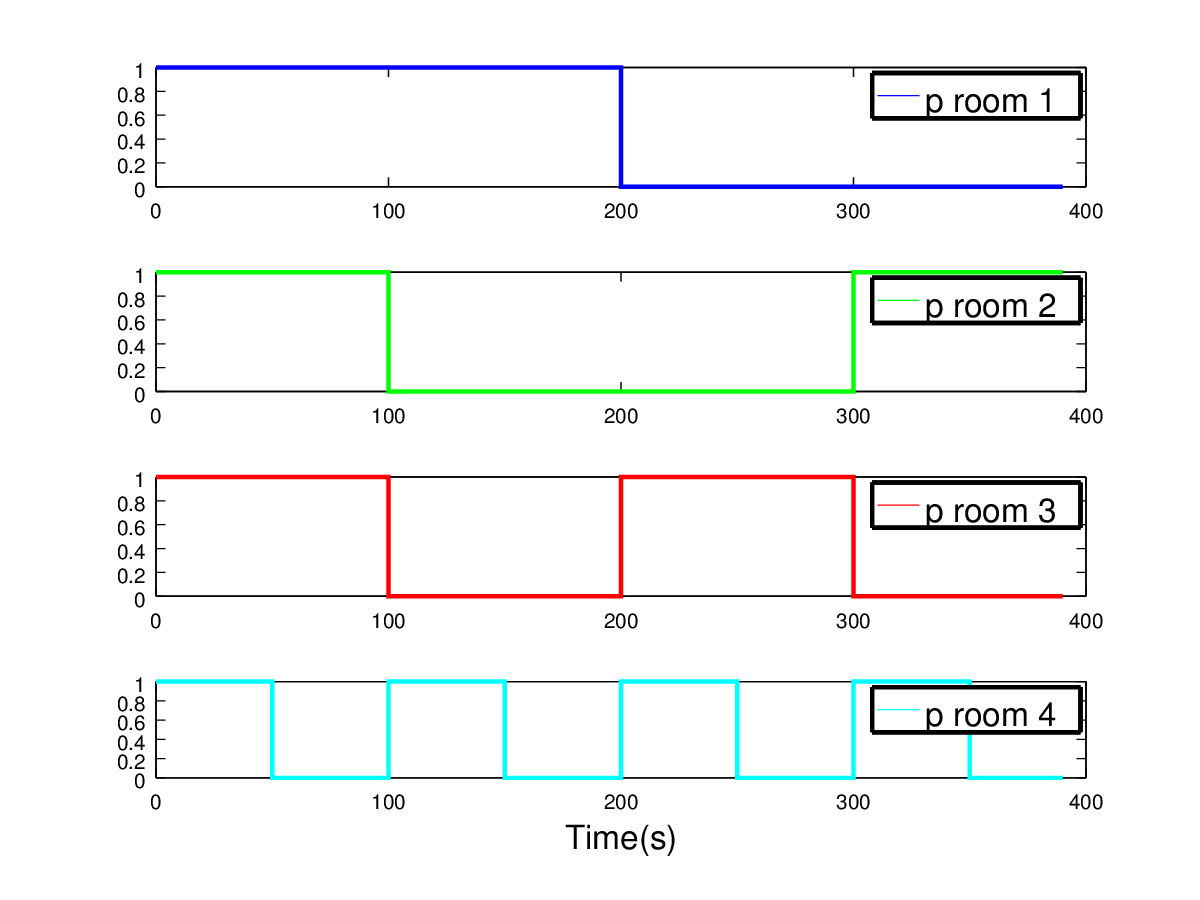
\includegraphics[scale=0.4]{NL_case_2_perturbation.png}
 \caption{Perturbation (presence of humans) imposed within time in the
   different rooms.}
  \label{fig:NL_2_part3_perturbation_part3}
\end{figure}


\begin{figure}[ht]
 \centering
 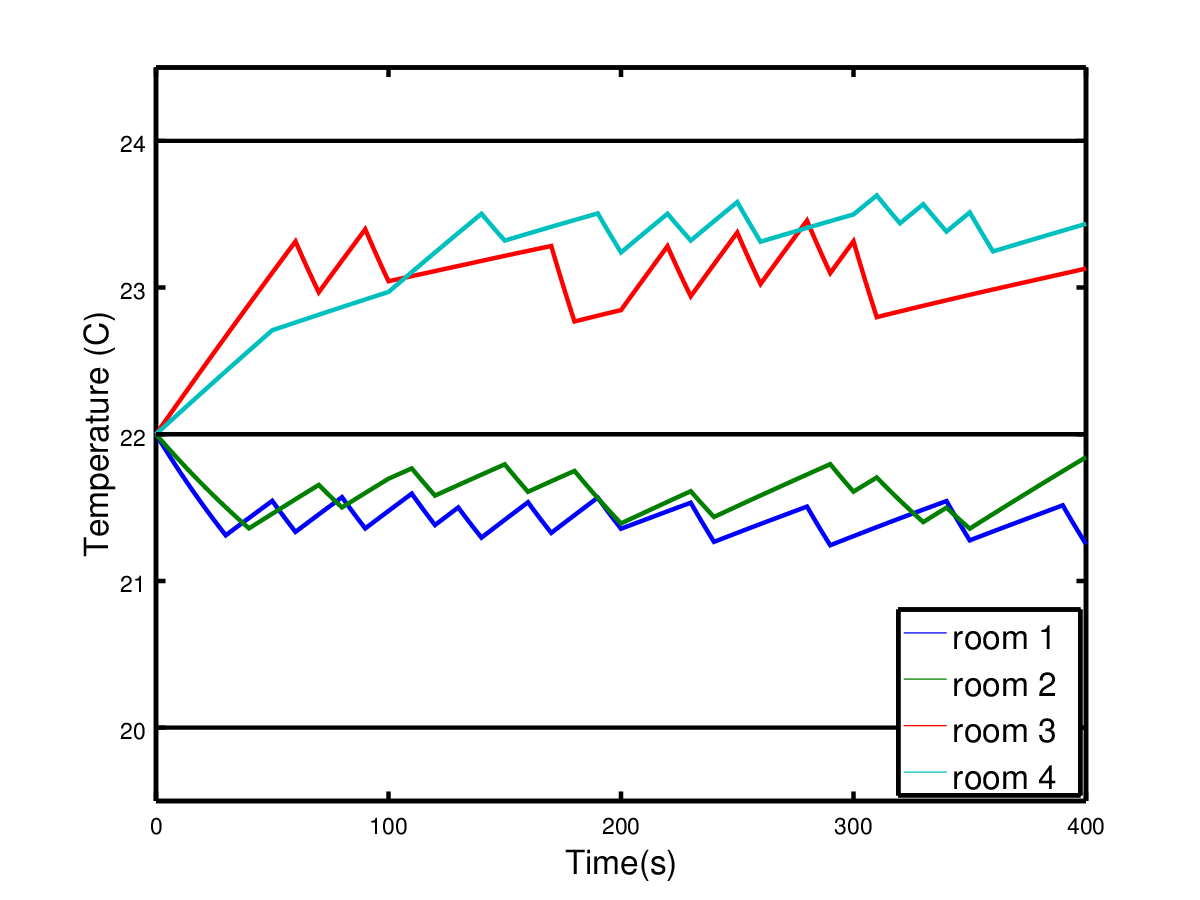
\includegraphics[scale=0.3]{compo_2objs2.png}%
% \caption{Simulation of the centralized controller from the initial condition $(22,22,22,22)$.}
%  \label{fig:NL_2_part3}
%\end{figure}
%
%\begin{figure}[ht]
% \centering
%\hfill
 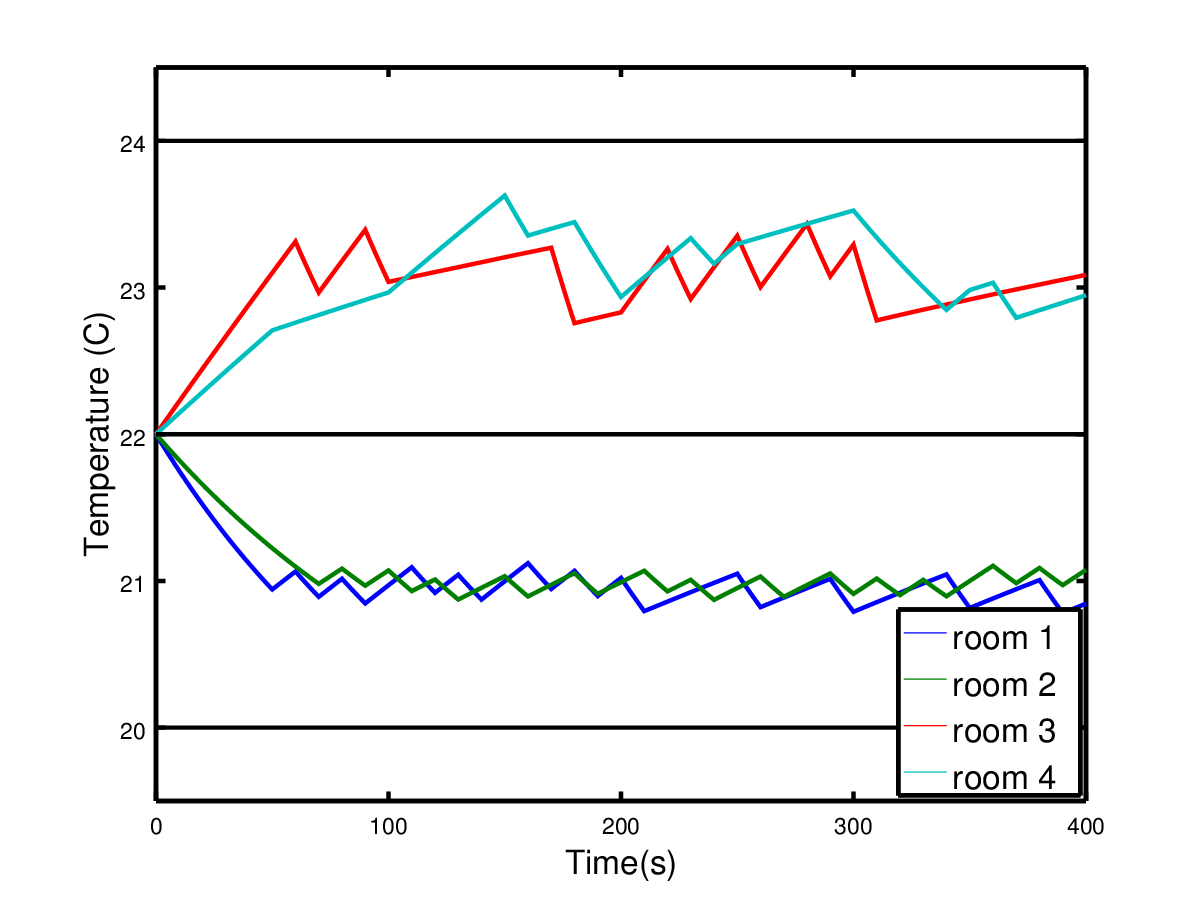
\includegraphics[scale=0.3]{compo_2objs3.png}
 \caption{Simulation of the centralized (left) and distributed (right) controllers from the initial condition $(22,22,22,22)$.}
  \label{fig:NL_2_part3}
\end{figure}

\subsection{Final Remarks}\label{sec:conc}

In this paper, we have proposed a distributed approach 
for control synthesis of sampled switching systems in the discrete-time framework
and applied it to a real floor heating system.
To our knowledge,
this is the first time that reachability and stability properties  
are guaranteed for a case study of this size. 
We have also explained how the method extends to the continuous-time framework.
The method can
be extended to take into account obstacles and safety constraints.

Note that it is essential in our method that the components are {\em sampled} with the {\em same} sampling period $\tau$, and that their clocks are synchronized.
It would be interesting to investigate how the approach behaves when clocks are badly synchronized or when they have different periods (see, e.g., \cite{KhatibGD16}).
%\fbox{Supprimer la phrase suivante, au moins...}
%We are currently investigating an 
%extension of the method to systems with non linear
%dynamics and varying parameters, see \cite{le2016control}. 




%\nocite{*}



